\documentclass[10pt,a4paper]{article}

\usepackage[margin=2cm]{geometry}
\usepackage{xcolor}
\usepackage{xurl}
%\usepackage{microtype}
%\microtypesetup{expansion=false}
\usepackage{titlesec}
\usepackage{cite}
\usepackage{url}
\usepackage[utf8]{inputenc}
\usepackage[T1]{fontenc}
\usepackage{lmodern}
\usepackage{booktabs}
\usepackage{caption}
\usepackage{graphicx}
\usepackage{float}
\graphicspath{{graphs/}}

\captionsetup[table]{labelfont=bf, font=small, skip=5pt}

\usepackage[
    colorlinks=true,
    linkcolor=blue,
    citecolor=blue,
    urlcolor=blue
]{hyperref}

\urlstyle{same}

\titlespacing*{\section}
  {0pt}
  {0.4cm}
  {0.2cm}
  
\titleformat{\section}
  {\normalfont\normalsize\bfseries}
  {\thesection.}
  {0.4em}
  {}
  
\titleformat{\subsection}
  {\normalfont\normalsize\bfseries}
  {\thesubsection}
  {0.2em}
  {}

\titlespacing*{\subsection}
  {0pt}
  {0.25cm}
  {0.15cm}

\setlength{\parindent}{1.5em}
\setlength{\parskip}{0pt}

\begin{document}

\thispagestyle{empty}

\vspace*{1.0cm}

\begin{center}
    {\Large Automatic Identification System (AIS)}\\[0.1cm]
    {\normalsize Introduction to Data Science with R and RStudio}

    \vspace{0.8cm}

    \begin{tabular}{c}
        \small Linus Schönewald, 974943, Digital Business Management\\
        \vspace{0.2cm}
        \small Robert Kaminski, 1100303, Information Systems\\
        \small \href{https://aidaho-edu.uni-hohenheim.de/gitlab/b0bat/aidaho_ids_thas_2026}{GitLab Repository}\\
        \small \href{http://193.197.231.174:7080/}{Dashboard}
    \end{tabular}

    \vspace{0.5cm}

    \small June, 2026
\end{center}

\vspace{0.5cm}

\hrule

\vspace{0.4cm}

\noindent\textbf{Abstract}

\vspace{0.2cm}

This report provides an overview of the Automatic Identification System (AIS) and the structure of the underlying vessel data.
After introducing the purpose and collection of AIS data, the report examines both static and dynamic vessel information.
Based on the available AIS database, different querying and sampling strategies are applied to explore vessel movements and traffic patterns.
The report further includes visual analyses of AIS observations, individual vessel behaviour, and spatial traffic density.
Finally, a static dashboard and an interactive Shiny application are implemented using Docker and NGINX.

\vspace{0.4cm}

\hrule

\vspace{0.2cm}

% ======================================================================================
% 1. Introduction
% ======================================================================================

\section{Introduction}

\vspace{0.2cm}

The Automatic Identification System (AIS) is a maritime communication system that allows 
vessels to automatically transmit and receive information about their identity, position, and movement \cite{1}.
Although AIS was initially introduced to improve navigational safety and support collision avoidance at sea, 
it has since become an important tool for maritime monitoring, fleet management, and maritime research \cite{2}.
Due to its importance for maritime safety and traffic monitoring, AIS carriage is mandatory under SOLAS 
(the International Convention for the Safety of Life at Sea) for certain vessel categories. This regulation requires
AIS on all ships of 300 gross tonnage and above engaged on international voyages, cargo ships of 500 gross tonnage 
and above not engaged on international voyages, and passenger ships regardless of size \cite{3}. AIS transponders are divided 
into Class A, mandatory for large vessels under SOLAS, and Class B, intended for smaller craft with limited functionality \cite{1}.

AIS data is collected by networks of receivers that capture Very High Frequency (VHF) radio waves transmitted by vessels.
As VHF radio signals are limited by distance, obstacles, and the Earth's curvature, AIS coverage depends strongly on
the location and height of the receiving antenna. In conventional ship-to-ship communication, AIS signals typically cover 
about 20 nautical miles, while shore-based AIS stations can extend this range to around 40 nautical miles. However, when AIS 
receivers are placed on satellites in low Earth orbit, the coverage range can increase significantly, reaching more than 1,000 
nautical miles. This makes satellite-based AIS particularly useful for long-range vessel identification and tracking, especially
in remote ocean areas where shore-based AIS stations cannot provide coverage \cite{4}. Despite this advantage, satellite-based AIS is 
inherently more vulnerable to message collisions than terrestrial AIS. While terrestrial AIS typically operates effectively in coastal 
waters due to its limited reception range and localized time-slot coordination, satellites cover much larger areas and can receive transmissions 
from hundreds of vessels simultaneously \cite{4,5}. As a result, multiple AIS messages may overlap in time and frequency, which can reduce decoding 
performance and lead to lost position reports \cite{5}.

In terms of transmitted information, AIS data are commonly divided into static, dynamic, and voyage-related information \cite{6}. Static information
includes vessel-specific identifiers and characteristics, such as the Maritime Mobile Service Identity (MMSI), call sign, vessel name, IMO number,
dimensions, and ship type \cite{1}. This data is usually configured during installation or system setup and transmitted every six minutes or upon request \cite{6}.
Dynamic information generally includes movement- and navigation-related data, such as the vessel's position, timestamp, course, speed, and heading \cite{1}. 
Most dynamic data, such as position, timestamp, speed, and course, are automatically updated by onboard systems, whereas navigational status is manually 
entered by the crew. The transmission frequency of dynamic information depends on the vessel's speed, course alterations, and AIS equipment type.
Voyage-related information, such as draught, destination, and estimated time of arrival, is also transmitted every six minutes or upon request, but it is 
manually entered and updated when necessary \cite{6}. Consequently, manually entered fields depend on regular human input and are generally more likely to be missing, 
incomplete, or outdated.

Taken together, the combination of dynamic movement information, static vessel characteristics, and voyage-related attributes makes AIS a highly valuable data source for 
the analysis of maritime traffic. Position, timestamp, speed, course, and heading allow vessel routes to be reconstructed and movement patterns to be examined in ports, 
waterways, and open-sea areas. When these dynamic records are linked with static vessel information, such as vessel type, flag, or dimensions, traffic patterns can also 
be compared across different vessel groups. However, the analytical value of AIS data is limited by their data quality. AIS datasets are often large and affected by missing,
duplicated, inaccurate, or outdated records. These issues may result from technical failures, limited receiver coverage, dense traffic, satellite message collisions, or 
incorrectly entered manual information. As a result, AIS data cannot be treated as a complete or error-free representation of vessel movement. They require systematic 
cleaning, validation, and plausibility checks before being used for maritime traffic analysis \cite{7}.

The aim of this report is to examine the analytical potential and limitations of AIS data for the study of vessel movement. AIS data provide detailed information about 
vessels, their characteristics, and their movement over time, but the size and quality of these datasets also create challenges for analysis. Therefore, 
the report considers how AIS data are structured, how large amounts of dynamic position data can be handled through sampling, and how spatial and temporal 
information can be used to study vessel behaviour. By using maps, plots, and dashboard elements, the project presents AIS-based traffic patterns in a clear way
while also showing that the results must be interpreted with attention to possible data quality issues.

% ======================================================================================
% 2. Data
% ======================================================================================

\section{Data}
The AIS vessel data was provided by \href{https://johannes-bleher.de/}{Dr. Bleher} via a PostgreSQL database, accessed through the PostgREST 
root endpoint at \url{https://aidaho-edu.uni-hohenheim.de/aisdb}. The API exposes ten queryable resources covering AIS records from 
January 1, 2021 to January 25, 2024.

\begin{table}[ht]
\caption{\textbf{Available PostgREST API resources.} The ten data tables and views exposed by the AIS database endpoint.}
\label{tab:api-resources}
\vspace{0.2cm}
\centering
\small
\begin{tabular}{@{}p{0.35\textwidth}p{0.55\textwidth}@{}}
\toprule
{\bfseries Endpoint} & {\bfseries Description} \\
\midrule
\texttt{ais\_static} & Static vessel information, one row per vessel \\
\texttt{ais\_dynamic} & Dynamic vessel information \\
\texttt{ais\_germany} & AIS records located within Germany \\
\texttt{geometry\_columns} & Metadata on geometry columns in the database \\
\texttt{germany\_h3} & H3 grid information for Germany \\
\texttt{ais\_dynamic\_daily\_counts} & Daily counts of dynamic AIS records \\
\texttt{geography\_columns} & Metadata on geography columns in the database \\
\texttt{ais\_dynamic\_daily\_counts\_mat} & Materialized daily counts of AIS records \\
\texttt{spatial\_ref\_sys} & Spatial reference system definitions \\
\texttt{ingested\_files} & Information on imported source files \\
\bottomrule
\end{tabular}
\end{table}

% ======================================================================================
% 2.1 Data Sources and Structure
% ======================================================================================

\subsection{Data Sources and Structure}

The AIS database consists of two central tables: \texttt{ais\_static} and \texttt{ais\_dynamic}. The \texttt{ais\_static} table
contains static vessel data, with one row per vessel identified by its MMSI. It contains 228,427 rows, representing unique vessel 
identifiers, and stores 13 columns. By contrast, the \texttt{ais\_dynamic} table contains dynamic vessel data and therefore multiple
observations per vessel over time. Due to the high-frequency transmission of AIS signals, the table contains approximately 826.79 million 
rows across 16 columns. Both tables are linked through the variable mmsi, which uniquely identifies vessels.
Table~\ref{tab:ais-static-variables} and Table~\ref{tab:ais-dynamic-variables} provide an overview of the columns contained in \texttt{ais\_static} and \texttt{ais\_dynamic} along with their meanings.
Beside these two central tables, the database also provides the table \texttt{ais\_germany}, which shares the same structure as \texttt{ais\_dynamic} 
but is restricted to vessels tracked within Germany, and later used for a German river traffic analysis.

\begin{table}[ht]
\caption{\textbf{Columns of the \texttt{ais\_static} table.} Field names, descriptions, and data types of the static, one-row-per-vessel metadata.}
\label{tab:ais-static-variables}
\vspace{0.2cm}
\centering
\small
\begin{tabular}{@{}p{0.22\textwidth}p{0.40\textwidth}p{0.30\textwidth}@{}}
\toprule
{\bfseries Column Name} & {\bfseries Description} & {\bfseries Type} \\
\midrule
\texttt{mmsi} & Maritime Mobile Service Identity (uniquely identifying a vessel) & \texttt{INTEGER} \\
\texttt{imo} & International Maritime Organization number & \texttt{INTEGER} \\
\texttt{name} & Vessel name & \texttt{TEXT} \\
\texttt{call\_sign} & Radio call sign & \texttt{TEXT} \\
\texttt{flag} & Country flag & \texttt{TEXT} \\
\texttt{draught} & Vessel draught in meters & \texttt{REAL} \\
\texttt{ship\_type\_code} & Numeric AIS ship type classification code & \texttt{SMALLINT} \\
\texttt{ship\_type} & Descriptive ship type category & \texttt{TEXT} \\
\texttt{length} & Length in meters & \texttt{REAL} \\
\texttt{width} & Width in meters & \texttt{REAL} \\
\texttt{eta} & Estimated time of arrival reported by the vessel & \texttt{TIMESTAMP WITH TIME ZONE} \\
\texttt{destination} & Destination reported by the vessel & \texttt{TEXT} \\
\texttt{static\_updated\_at} & Timestamp of last static information update & \texttt{TIMESTAMP WITH TIME ZONE} \\
\bottomrule
\end{tabular}
\end{table}


\begin{table}[ht]
\caption{\textbf{Columns of the \texttt{ais\_dynamic} table.} Field names, descriptions, and data types of the dynamic position messages.}
\label{tab:ais-dynamic-variables}
\vspace{0.2cm}
\centering
\small
\begin{tabular}{@{}p{0.22\textwidth}p{0.40\textwidth}p{0.30\textwidth}@{}}
\toprule
{\bfseries Column Name} & {\bfseries Description} & {\bfseries Type} \\
\midrule
\texttt{created\_at} & Timestamp when the record was ingested & \texttt{TIMESTAMP WITH TIME ZONE} \\
\texttt{msg\_timestamp} & Timestamp of the original AIS message & \texttt{TIMESTAMP WITH TIME ZONE} \\
\texttt{position\_updated\_at} & Timestamp when the vessel position was last updated & \texttt{TIMESTAMP WITH TIME ZONE} \\
\texttt{mmsi} & Maritime Mobile Service Identity (uniquely identifying a vessel) & \texttt{INTEGER} \\
\texttt{latitude} & Geographic latitude in decimal degrees & \texttt{DOUBLE PRECISION} \\
\texttt{longitude} & Geographic longitude in decimal degrees & \texttt{DOUBLE PRECISION} \\
\texttt{speed} & Speed over ground (SOG) in knots & \texttt{REAL} \\
\texttt{course} & Course over ground (COG) in degrees & \texttt{REAL} \\
\texttt{heading} & Heading in degrees & \texttt{SMALLINT} \\
\texttt{status} & Navigational status code reported by the vessel & \texttt{SMALLINT} \\
\texttt{maneuver} & Maneuver indicator reported by the vessel & \texttt{SMALLINT} \\
\texttt{accuracy} & Accuracy of the reported position & \texttt{BOOLEAN} \\
\texttt{rot} & Rate of turn (ROT) & \texttt{SMALLINT} \\
\texttt{collection\_type} & Source of data collection & \texttt{TEXT} \\
\texttt{geom} & Geographic point geometry of the position & \texttt{PUBLIC.GEOGRAPHY(POINT,4326)} \\
\texttt{h3\_index} & H3 grid index assigned to the vessel position & \texttt{BIGINT} \\
\bottomrule
\end{tabular}
\end{table}

% ======================================================================================
% 2.2 Coverage and Limitations
% ======================================================================================

\subsection{Limitations}

Although the introduction already outlined general limitations of AIS data, they are
worth reconsidering for the database used here, as they directly affect the
completeness and reliability of the analysis.

Coverage must be considered in two ways. First, AIS reception depends on the receiver
infrastructure: terrestrial reception is strongest near coasts, ports, and inland
waterways, while satellite AIS covers much larger areas but suffers message collisions
in dense-traffic zones, where overlapping transmissions are not reliably decoded \cite{4,5}.
Second, this creates availability bias --- the recorded observations are not a random
draw from all transmissions but reflect what the infrastructure was most likely to
capture \cite{8}. Coastal cargo traffic, ferries, and port approaches are therefore
over-represented, while offshore fishing, remote routes, and polar regions appear less
often or with larger gaps. The database should thus be read as a coverage-dependent
sample, not a complete or unbiased record of all vessel movement.

AIS data may also contain erroneous records. Raw data include invalid, abnormal, or
duplicated values (``dirty'' data) caused by interference, equipment faults, or device
manipulation \cite{9}, which can produce incorrect positions, artificial jumps, or
implausible speeds \cite{10}. A further problem is identifier reuse: because tracks are
reconstructed from the MMSI, a shared MMSI makes a track jump between locations in a
characteristic zigzag \cite{9,10}. Unusual routes or extreme speeds should therefore be
interpreted with caution, as they may reflect data errors rather than real behaviour.

Finally, the dataset is far too large to process in full, so the analysis necessarily
relies on filtered extracts and samples \cite{11}. The results therefore depend not only on
the underlying data but also on the specific queries, sampling strategy, and extraction
criteria used.

These limitations shape the interpretation of the results. The following analyses therefore need to be understood as being based on selected, coverage-dependent records 
that may contain gaps, errors, and biases caused by both the data collection process and the practical limits of working with a large shared database.

% ======================================================================================
% 3. Descriptive Overview
% ======================================================================================

\section {Descriptive Overview}

Before analysing vessel movements, it is important to examine the structure and quality of the AIS static information.
Several patterns are visible in the numeric variables, as shown in Table~\ref{tab:numeric-summary}. The minimum of 0 across all variables is physically not possible,
suggesting that some entries use 0 as a placeholder for missing information. In addition, the mean exceeds the median for 
all three variables, indicating right-skewed distributions. This is especially visible for length, where the maximum value of 
1,022 meters is physically implausible and suggests the presence of erroneous outliers. While length and width are relatively 
complete, draught is missing for approximately 47\% of the observations, limiting its usefulness for further analysis.

\begin{table}[ht]
\caption{\textbf{Numeric summary of \texttt{ais\_static}.} Minimum, mean, median, maximum, and non-missing count for the numeric vessel attributes.}
\label{tab:numeric-summary}
\vspace{0.2cm}
\centering
\small
\begin{tabular}{@{}lrrrrr@{}}
\toprule
{\bfseries Variable} & {\bfseries Min} & {\bfseries Mean} & {\bfseries Median} & {\bfseries Max} & {\bfseries NonMissing} \\
\midrule
draught & 0 & 4.7158  &  4 &   25.5 & 121121 \\
length  & 0 & 63.5805 & 32 & 1022.0 & 216537 \\
width   & 0 & 11.5478 &  8 &  126.0 & 216537 \\
\bottomrule
\end{tabular}
\end{table}

The categorical variables also show strong concentration and varying levels of reliability. As shown in Table~\ref{tab:overview-ship-types}, the dataset includes
a wide range of ship types, but the distribution is clearly dominated by a few categories, particularly Cargo vessels (25.1\%) and Fishing vessels (16.8\%).
This dominance is likely related to terrestrial receiver coverage near coasts and ports, combined with SOLAS carriage requirements that mandate AIS for 
larger cargo vessels \cite{3}. At the same time, the category Other accounts for the largest share of observations (28.1\%), showing the diversity of ship types in 
the dataset that occur too infrequently to be represented as separate classes. In addition, a substantial number of records contain missing ship type 
information (n = 21,842), corresponding to approximately 9.6\% of all observations. This should be considered when interpreting the results, as missing 
values may limit the reliability of conclusions based on ship type.

\begin{table}[ht]
\caption{\textbf{Ship types in \texttt{ais\_static}.} Frequency and share of each vessel type; percentages exclude the 21,842 records with no reported type.}
\label{tab:overview-ship-types}
\vspace{0.2cm}
\centering
\small
\begin{tabular}{@{}lrr@{}}
\toprule
{\bfseries Ship Type} & {\bfseries Frequency} & {\bfseries Percentage (\%)} \\
\midrule
Other              & 57,974 & 28.1 \\
Cargo              & 51,781 & 25.1 \\
Fishing Vessel     & 34,736 & 16.8 \\
Tanker             & 16,496 &  8.0 \\
Tug                & 13,257 &  6.4 \\
Pleasure Craft     &  9,014 &  4.4 \\
Special Craft      &  7,624 &  3.7 \\
Passenger Ship     &  7,147 &  3.5 \\
Sailing Vessel     &  5,164 &  2.5 \\
High-Speed Craft   &  1,227 &  0.6 \\
Search and Rescue  &  1,201 &  0.6 \\
Wing In Ground     &    644 &  0.3 \\
Reserved           &    320 &  0.2 \\
\midrule
\multicolumn{3}{l}{Percentages are calculated excluding NA values (n = 21,842)} \\
\bottomrule
\end{tabular}
\end{table}

Although the dataset contains vessels operating under 229 distinct national flags (a
further 22 vessels report no flag), the distribution is highly concentrated. As shown
in Table~\ref{tab:overview-flags}, Chinese-flagged vessels alone account for almost
30\% of all vessels --- nearly five times the share of the next most common flag (the
United States, 6.0\%). Consistent with this pattern, the most common destinations are
located in China. However, the destination variable is not consistently usable because
over 50\% of the entries are either missing or appear to be erroneous. Many records
contain only placeholders, such as repeated ``@'' symbols, while others contain broad
route descriptions rather than standardised destination names, for example
``FOR ORDERS''. This is likely because destination information is manually entered and
therefore likely to contain inconsistent formatting, missing values, and input errors.

\begin{table}[ht]
\caption{\textbf{Most common flags in \texttt{ais\_static}.} The five most frequent national flags and their share of all 228,427 vessels.}
\label{tab:overview-flags}
\vspace{0.2cm}
\centering
\small
\begin{tabular}{@{}lrr@{}}
\toprule
{\bfseries Flag} & {\bfseries Frequency} & {\bfseries Percentage (\%)} \\
\midrule
CN & 67,214 & 29.4 \\
US & 13,771 &  6.0 \\
PA &  8,024 &  3.5 \\
NL &  7,635 &  3.3 \\
NO &  7,303 &  3.2 \\
\midrule
\multicolumn{3}{l}{Five most common of 229 flags; percentages are of all 228,427 vessels} \\
\bottomrule
\end{tabular}
\end{table}

% ======================================================================================
% 3.x Targeted Filter Queries (Task 2.4)
% ======================================================================================

\subsection{Targeted Filter Queries}

Beyond these aggregate overviews, the PostgREST interface allows specific subsets of
the data to be retrieved by combining filters in the request URL. Filters are
AND-combined, and counts were obtained with the same exact-count method used for the
table sizes (a \texttt{HEAD} request with \texttt{Prefer: count=exact}), so no row data
has to be transferred. Table~\ref{tab:filter-queries} reports several such queries
together with the filter logic used.

\begin{table}[H]
\caption{\textbf{Targeted filter queries.} Results of combined PostgREST filters against the AIS tables, with the filter logic used.}
\label{tab:filter-queries}
\vspace{0.2cm}
\centering
\small
\begin{tabular}{@{}p{5.1cm}p{6.1cm}r@{}}
\toprule
{\bfseries Query} & {\bfseries PostgREST filter} & {\bfseries Result} \\
\midrule
Benelux-flagged vessels                 & \texttt{flag=in.(BE,NL,LU)}                       & 9,476 \\
German cargo vessels                    & \texttt{flag=eq.DE} \& \texttt{ship\_type=eq.Cargo} & 291 \\
\quad of those longer than 150\,m       & \texttt{\dots \& length=gt.150}                   & 76 \\
Name contains ``EXPRESS''               & \texttt{name=ilike.*EXPRESS*}                     & 572 \\
Dynamic records, first 5\,min of 2022   & \texttt{msg\_timestamp} in 5-min window           & 1,506 \\
\quad distinct vessels therein          & distinct \texttt{mmsi}                            & 1,100 \\
Faster than 12\,kn (2021-05-04, 14:00--14:30) & \texttt{speed=gt.12}                         & 76 \\
\quad of those cargo                    & cross-referenced with \texttt{ais\_static}        & 31 \\
\bottomrule
\end{tabular}
\end{table}

In total, 9,476 vessels sail under a Benelux flag, and 291 German-flagged cargo vessels
are recorded, of which 76 exceed 150~m in length. A case-insensitive name search returns
572 vessels whose name contains ``EXPRESS''. On the dynamic side, the first five minutes
of 2022 contain 1,506 position records from 1,100 distinct vessels, and within the
30-minute window on 2021-05-04, 76 vessels moved faster than 12~knots, of which 31 are
cargo vessels. The number of returned rows is itself controlled with the
\texttt{limit} parameter (for example \texttt{limit=5}), which is used throughout to
keep responses within the API's size limit.

% ======================================================================================
% 4. Sampling Strategy
% ======================================================================================

\section {Sampling Strategy}

Because the full AIS dynamic table contains several hundred million records, it is not realistic to analyse the complete
dataset within this project. For this reason, a sample had to be selected.

A sampling strategy is a method for selecting a smaller representative sample from a larger dataset. Sampling
is often necessary because full datasets can be too large, costly, and slow to process. However, sampling is not
simply the act of using less data. A sample should preserve the relevant structure of the population so that
analysis on the sample leads to conclusions that remain meaningful for the larger dataset \cite{12}.
Good sampling should therefore be:

\begin{itemize}
    \item \texttt{Representative}: Sample reflects the dataset it was drawn from.
    \item \texttt{Unbiased}: No subgroup is over- or under-represented due to the selection mechanism.
    \item \texttt{Reproducible}: Same sample can be reconstructed.
    \item \texttt{Appropriately sized}: Large enough to draw reliable conclusions.
\end{itemize}

A sample is representative if the statistical feature of the variables, such as distribution, mean, correlations,
rare events, etc., are similar to those of the entire dataset. Since the AIS API contains a very large amount
of data, sampling is essential. However, AIS samples can become non-representative in several ways. The
important dimensions of possible non-representativeness are:

\begin{itemize}
    \item \texttt{Geographical bias}: The sample could mostly contain data around high-traffic areas, under representing
                  data from the open ocean or less-frequent areas.
    \item \texttt{Temporal bias}: The sample could be only from certain days, seasons, or hours may miss daily, weekly,
                  or seasonal traffic patterns. Furthermore, sampling by taking every n-th ping can disrupt the vessel's
                  continuous path, reducing accuracy of speed, acceleration, etc.
    \item \texttt{Vessel bias}: The sample could be biased by vessel type or behaviour. For example, large commercial
                  vessels may be over-represented because they transmit regularly and travel through monitored shipping
                  lanes, while small fishing vessels or vessels with irregular transmissions may be under-represented.
\end{itemize}

In addition to these sampling biases, the previously mentioned availability bias must be considered again in 
the context of the sampling strategy \cite{8}. AIS data is not collected uniformly from all vessels and regions, but depend on the underlying collection infrastructure \cite{4,5}.
Therefore, the available database already represents a coverage-dependent subset of all possible AIS transmissions. If a sample is drawn directly from this 
database without considering variables such as region, time period, vessel type, or collection type, the sample may reproduce or even strengthen this availability bias.
As a result, the sampling strategy should not only reduce the dataset size, but also check whether important spatial, temporal, and vessel-related structures remain 
represented.

To address these challenges, two sampling strategies were implemented and compared to select 10,000 AIS
observations from the millions of records available for January 24, 2024.

% ======================================================================================
% 4.1 Interval-Based Sample
% ======================================================================================

\subsection{Interval-Based Sample}

The first approach was cluster sampling, which involves dividing the population into groups (clusters) and
randomly selecting a subset of these groups for sampling \cite{12}. So each 5-minute interval on January 24, 2024,
was treated as a cluster. A total of 100 intervals were randomly selected, and up to 100 AIS observations were
extracted from each interval until a sample size of 10,000 observations was reached. But this strategy may
introduce several biases. First, it is vulnerable to the temporal bias, as the randomly selected intervals may
not fully capture traffic patterns throughout the day. As a result, periods with unusually high or low vessel
activity could be over- or under-represented in the sample. Secondly, geographical bias may occur because
vessel activity is not evenly distributed across space. Observations from busy ports and major shipping routes
may be sampled more often than observations from remote offshore areas, reducing the representativeness of
the sample.

% ======================================================================================
% 4.2 Stratified Sampling
% ======================================================================================

\subsection{Stratified Sampling}

Given the potential biases associated with cluster sampling, a stratified sampling approach was used next.
Unlike cluster sampling, stratified sampling divides the population into subgroups (strata) based on shared
traits and draws observations from each subgroup in proportion to its size in the population \cite{8}. The data were
divided into strata based on ship type and hour of day. Observations were then allocated proportionally across
strata and retrieved separately, ensuring that larger groups contributed more records while smaller groups
remained represented. The corresponding proportional allocation is reported in
Table~\ref{tab:stratified-allocation}. Because PostgREST offers no true random-row
operator, randomness within each stratum was approximated in two stages: vessels were
drawn at random from the stratum and their records were then randomly subsampled in R
to the allocated count, with a fixed seed (\texttt{set.seed(2026)}) keeping the draw
reproducible.

\begin{table}[ht]
\caption{\textbf{Stratified allocation of 10,000 observations.} Records on 24 January 2024 and the resulting proportional allocation, aggregated by ship type.}
\label{tab:stratified-allocation}
\vspace{0.2cm}
\centering
\small
\begin{tabular}{@{}lrr@{}}
\toprule
{\bfseries Ship type} & {\bfseries Records (Jan 24)} & {\bfseries Allocation} \\
\midrule
Cargo             & 21,036,091 & 3,305 \\
Tanker            & 10,688,122 & 1,686 \\
Other             &  8,879,565 & 1,401 \\
Fishing Vessel    &  6,197,875 &   979 \\
Tug               &  5,698,967 &   900 \\
Passenger Ship    &  2,796,149 &   440 \\
Special Craft     &  2,766,002 &   438 \\
(not reported)    &  1,845,297 &   292 \\
Pleasure Craft    &  1,512,689 &   238 \\
Sailing Vessel    &    727,607 &   117 \\
High-Speed Craft  &    589,924 &    95 \\
Wing In Ground    &    234,093 &    43 \\
Search and Rescue &    234,824 &    42 \\
Reserved          &    130,036 &    24 \\
\bottomrule
\end{tabular}
\end{table}

% ======================================================================================
% 4.3 Comparison
% ======================================================================================

\subsection{Comparison}

To evaluate the representativeness of both samples, the distributions of ship type, speed, and collection type
were compared.

Regarding ship type, the stratified sample contains a substantially larger proportion of commercial vessel types
such as cargo ships and tankers, while the interval sample contains relatively more smaller or specialised vessels,
as shown in Figure~\ref{fig:shipcompare}. This is consistent with the temporal bias described above. By
randomly selecting time windows, the interval sample may have captured periods of atypical vessel activity,
leading to an over-representation of smaller and specialised vessels.

\begin{figure}[H]
    \centering
    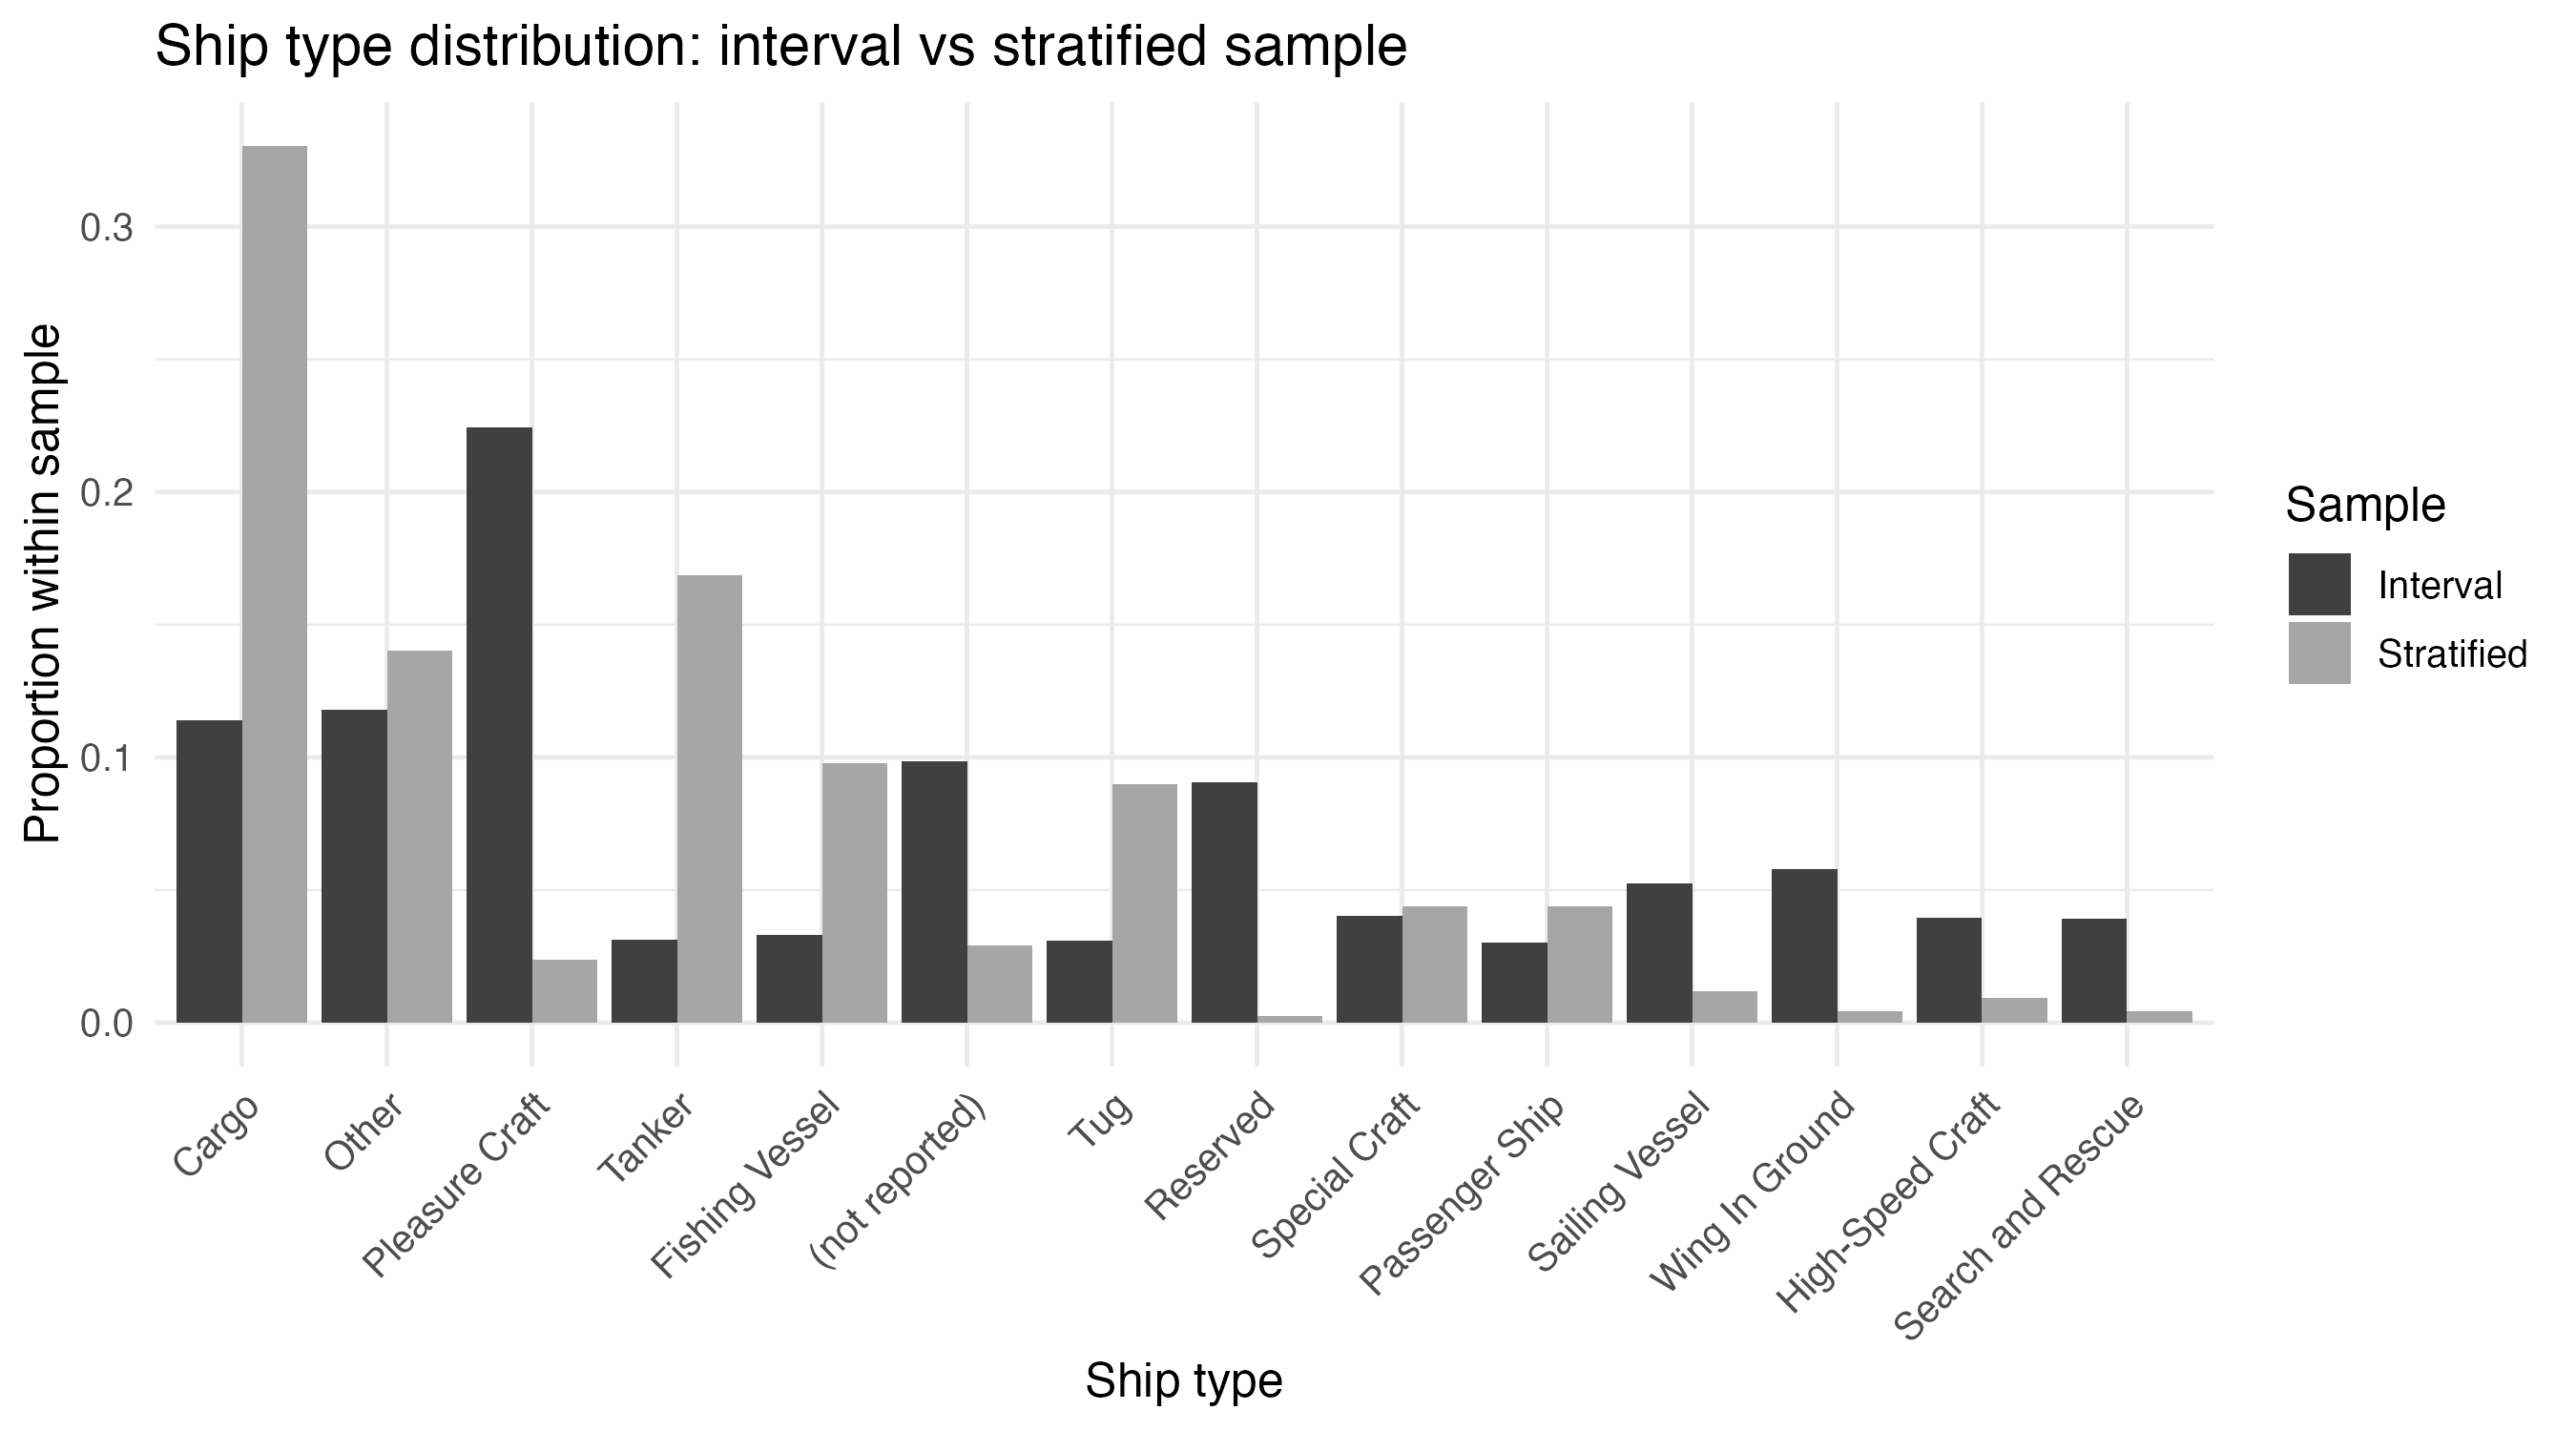
\includegraphics[width=0.85\textwidth]{compare_ship_type.png}
    \caption{\textbf{Ship-type distribution by sample.} Proportion of each ship type in the interval and stratified samples.}
    \label{fig:shipcompare}
\end{figure}

Figure~\ref{fig:collectioncompare} compares the collection-type distribution of the interval and stratified samples. As mentioned before, 
Class A mainly refers to AIS transponders used by larger vessels under SOLAS, while Class B is mainly used by smaller vessels with more limited functionality \cite{1}.
Both samples are dominated by dynamic\_classA. However, the stratified sample contains a lower share of dynamic\_classB observations and a higher share of satellite 
observations. This is likely because stratified sampling reflects the overall structure of the dataset more closely, especially the strong presence of cargo ships and 
tankers, which are often linked to Class A and satellite-based AIS records.

\begin{figure}[H]
    \centering
    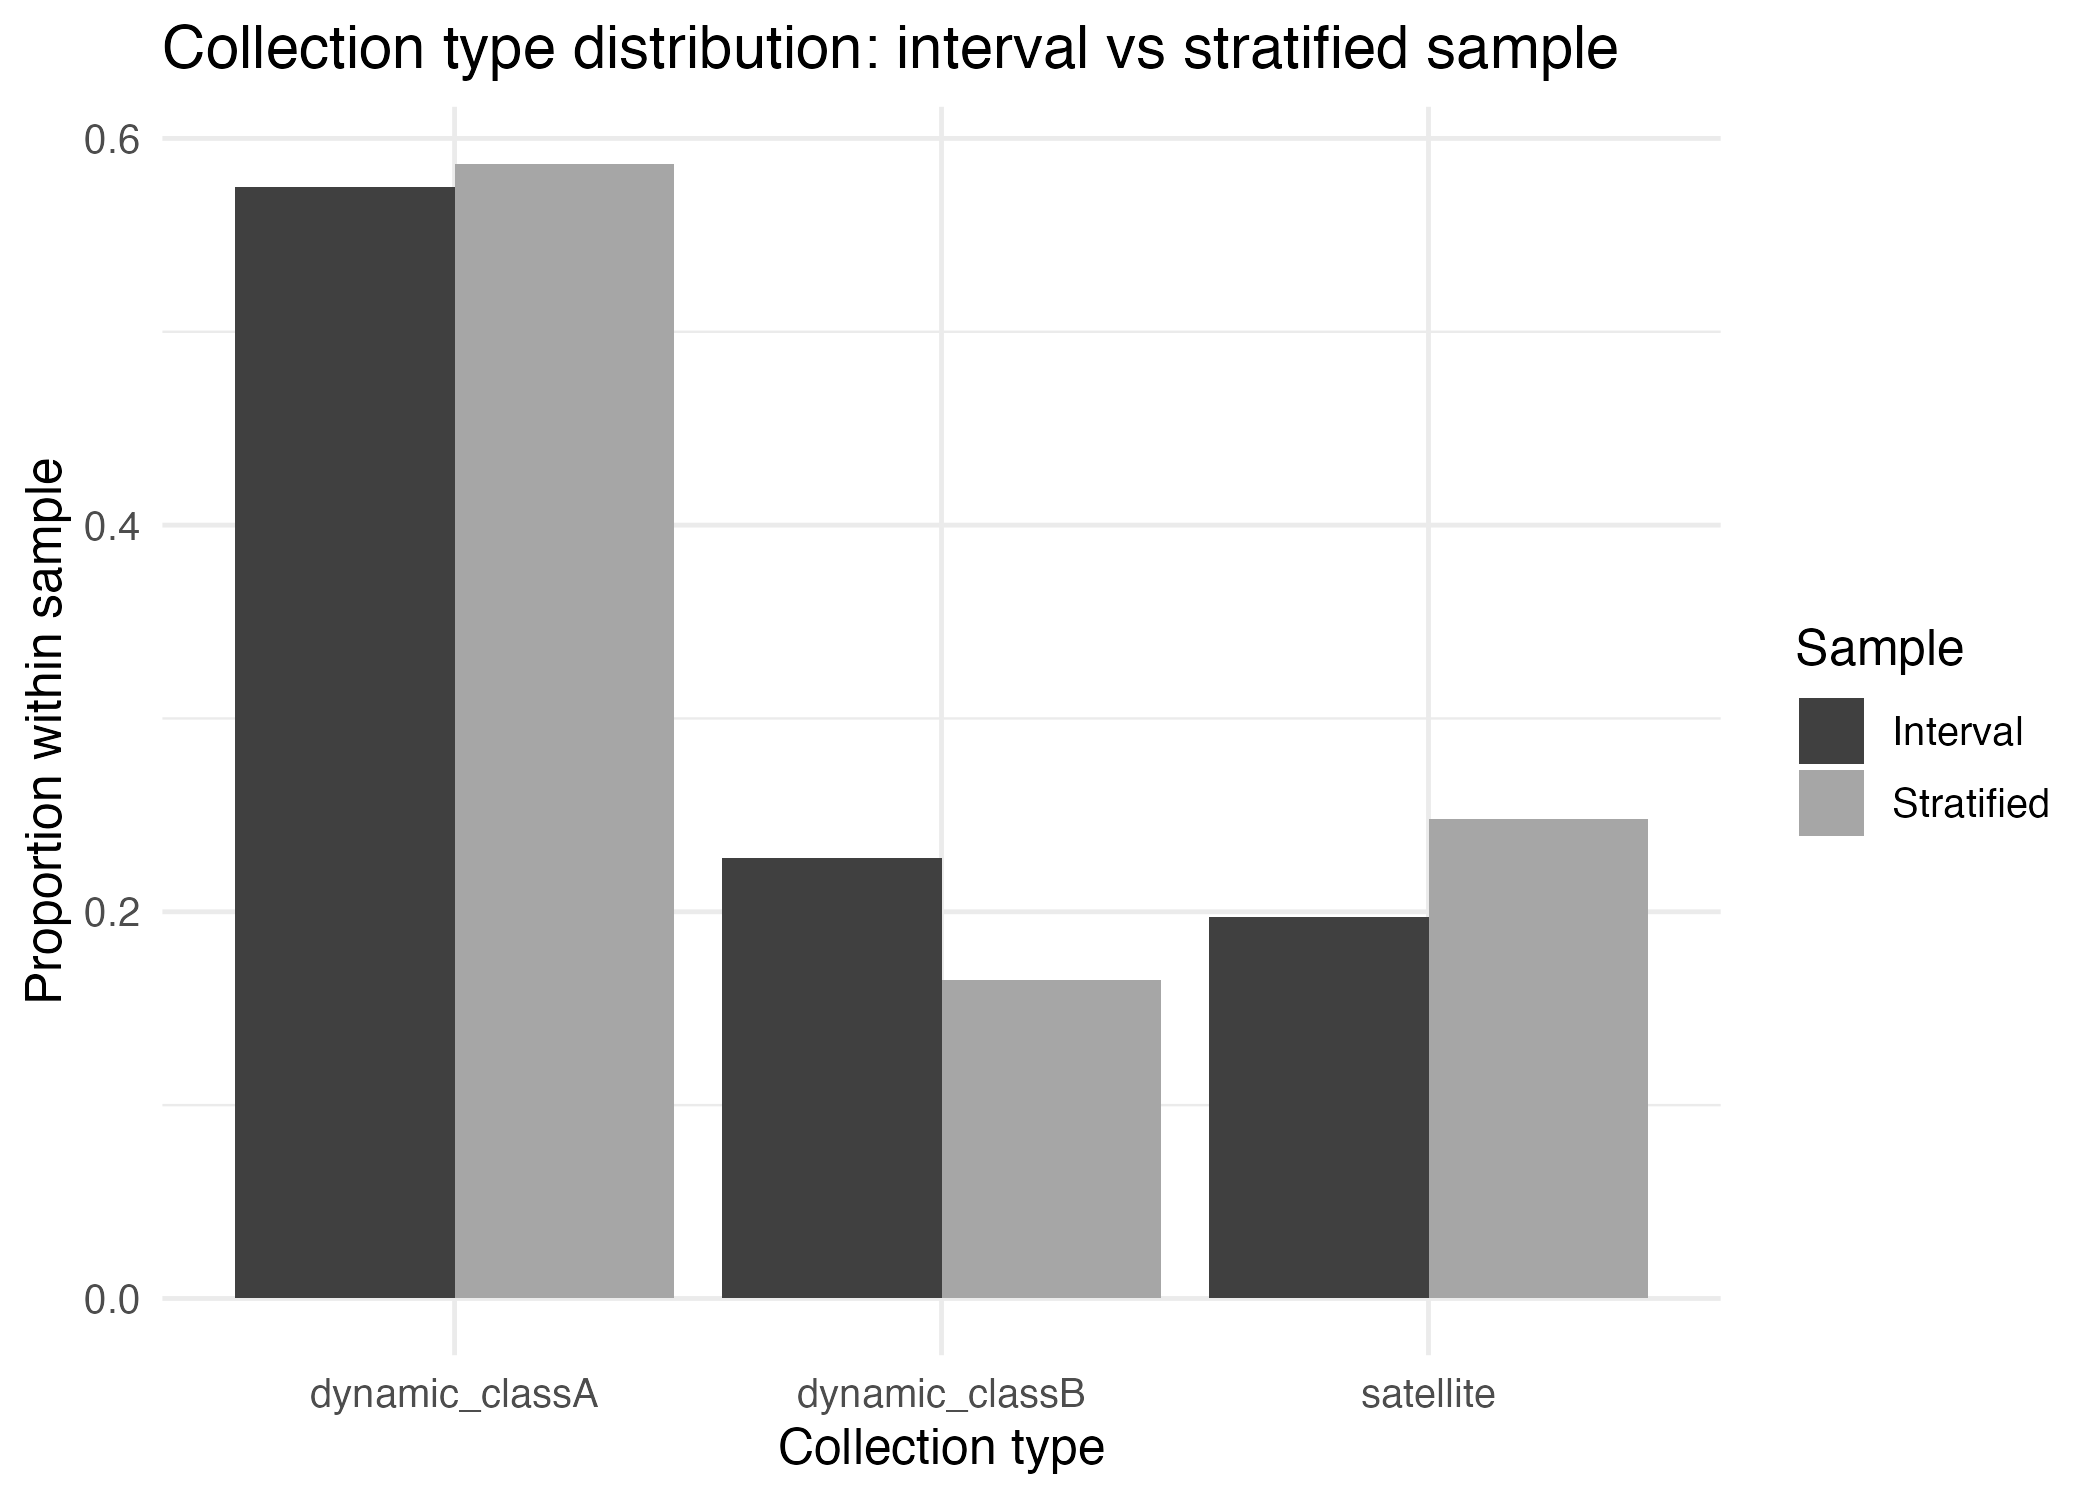
\includegraphics[width=0.65\textwidth]{compare_collection_type.png}
    \caption{\textbf{Collection-type distribution by sample.} Proportion of each collection type (Class A, Class B, satellite) in the two samples.}
    \label{fig:collectioncompare}
\end{figure}

Figure~\ref{fig:speedcompare} makes the weakness of the interval-based sample even more clear. The interval sample is strongly concentrated at very low speeds, meaning that it includes 
too many stationary or very slow-moving vessels. This makes it less reliable for analysing general vessel movement, because it does not represent the full speed 
structure very well. The stratified sample, on the other hand, shows a broader distribution and includes more vessels at medium speeds, especially around 10 to 12 knots. 
This suggests that it captures moving vessel traffic more realistically.

\begin{figure}[H]
    \centering
    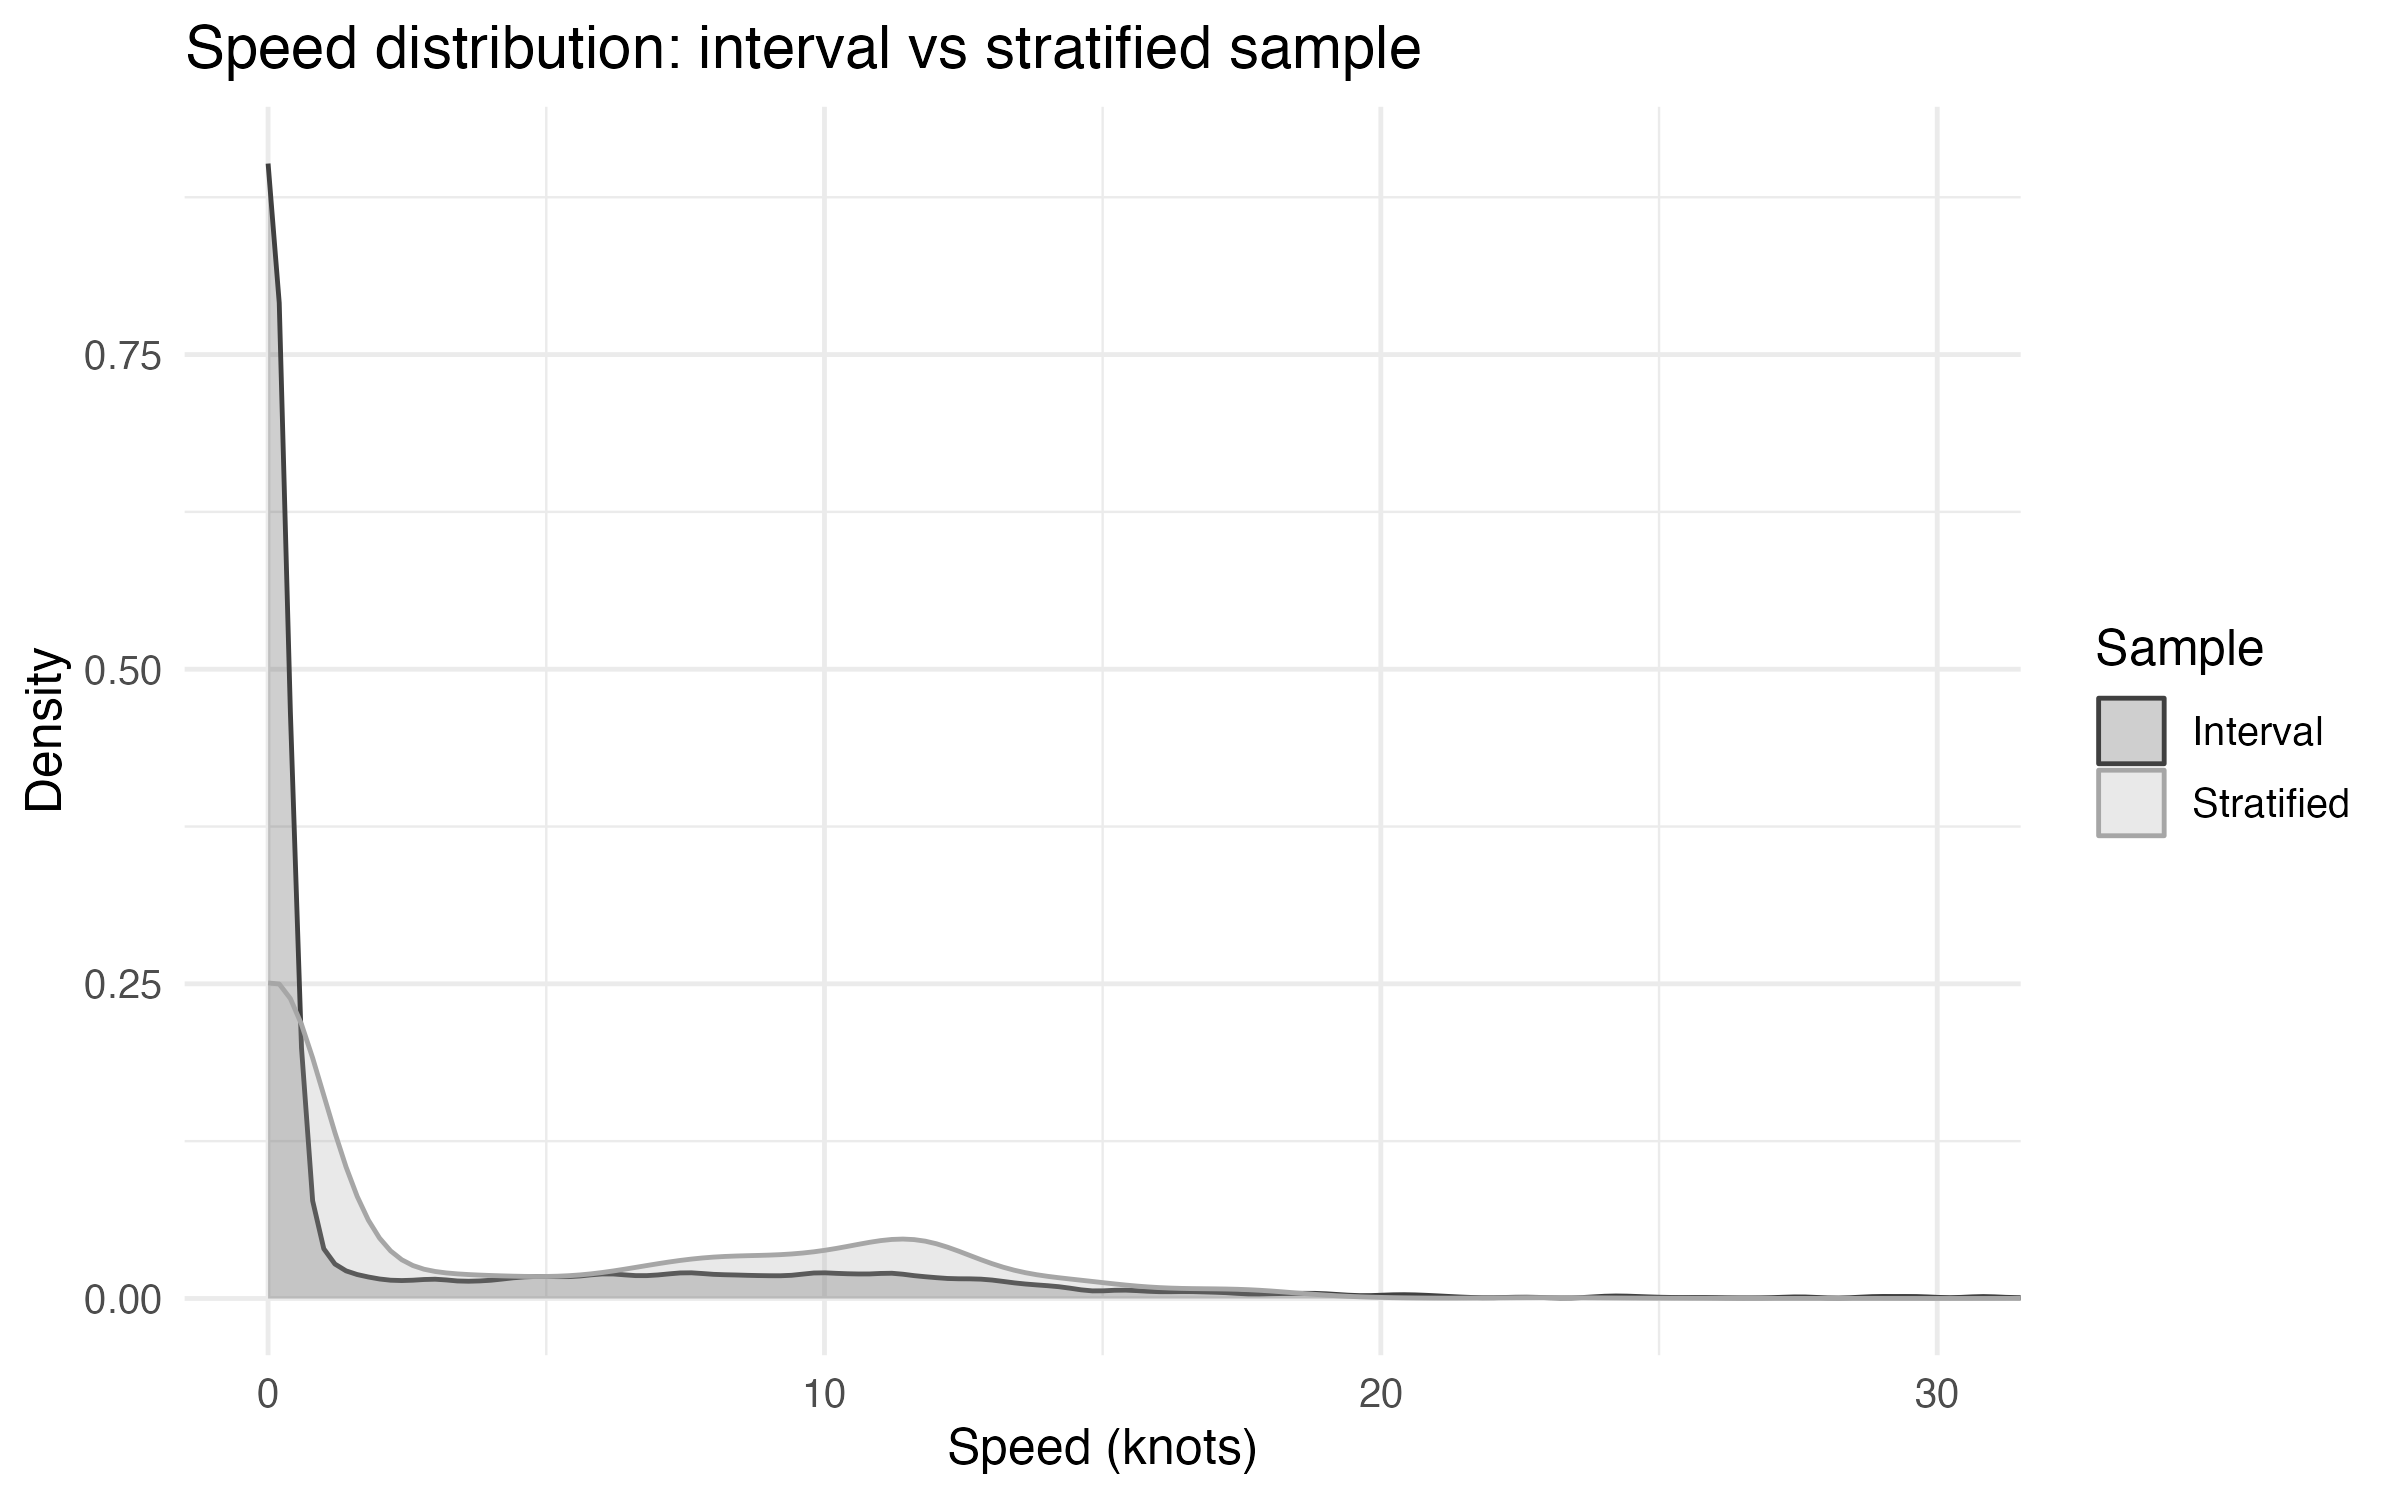
\includegraphics[width=0.75\textwidth]{compare_speed.png}
    \caption{\textbf{Speed distribution by sample.} Kernel density of speed over ground for the interval and stratified samples.}
    \label{fig:speedcompare}
\end{figure}

Overall, the comparison shows that the interval-based sample is strongly affected by the randomly selected time windows. 
This can lead to an over-representation of specific traffic situations, such as slow-moving vessels or periods with more 
smaller and specialised vessels. Therefore, the interval-based sample shows a clear risk of temporal bias. The stratified sample gives a more 
balanced picture because it better preserves differences between ship types and hours of the day. As a result, the interval-based sample is 
easier to construct, but it is less representative than the stratified sample.

% ======================================================================================
% 5. Vessel Behaviour
% ======================================================================================

\section {Vessel Behaviour}

This section moves from aggregate statistics to the behaviour of individual
vessels. It first gives a visual overview of the sampled AIS positions, then
inspects three specific vessels to illustrate both data-quality problems and
characteristic movement patterns, and finally develops a rule-based method for
detecting ship-lock passages from a vessel track.

% ======================================================================================
% 5.1 Sample Overview Maps
% ======================================================================================

\subsection {Sample Overview Maps}

To provide a visual overview of the AIS data, Figure~\ref{fig:map-full} maps all AIS
positions worldwide from the previously created cluster sample. Vessel speed is
represented by colour using a sequential scale capped at 25 knots, with pale yellow
indicating lower speeds and dark red indicating higher speeds; the cap prevents a few
implausibly high speeds from compressing the colour scale. Most observations are
concentrated along major shipping routes and coastal regions, particularly around
Europe, East Asia, North America, and the Mediterranean Sea.

\begin{figure}[H]
    \centering
    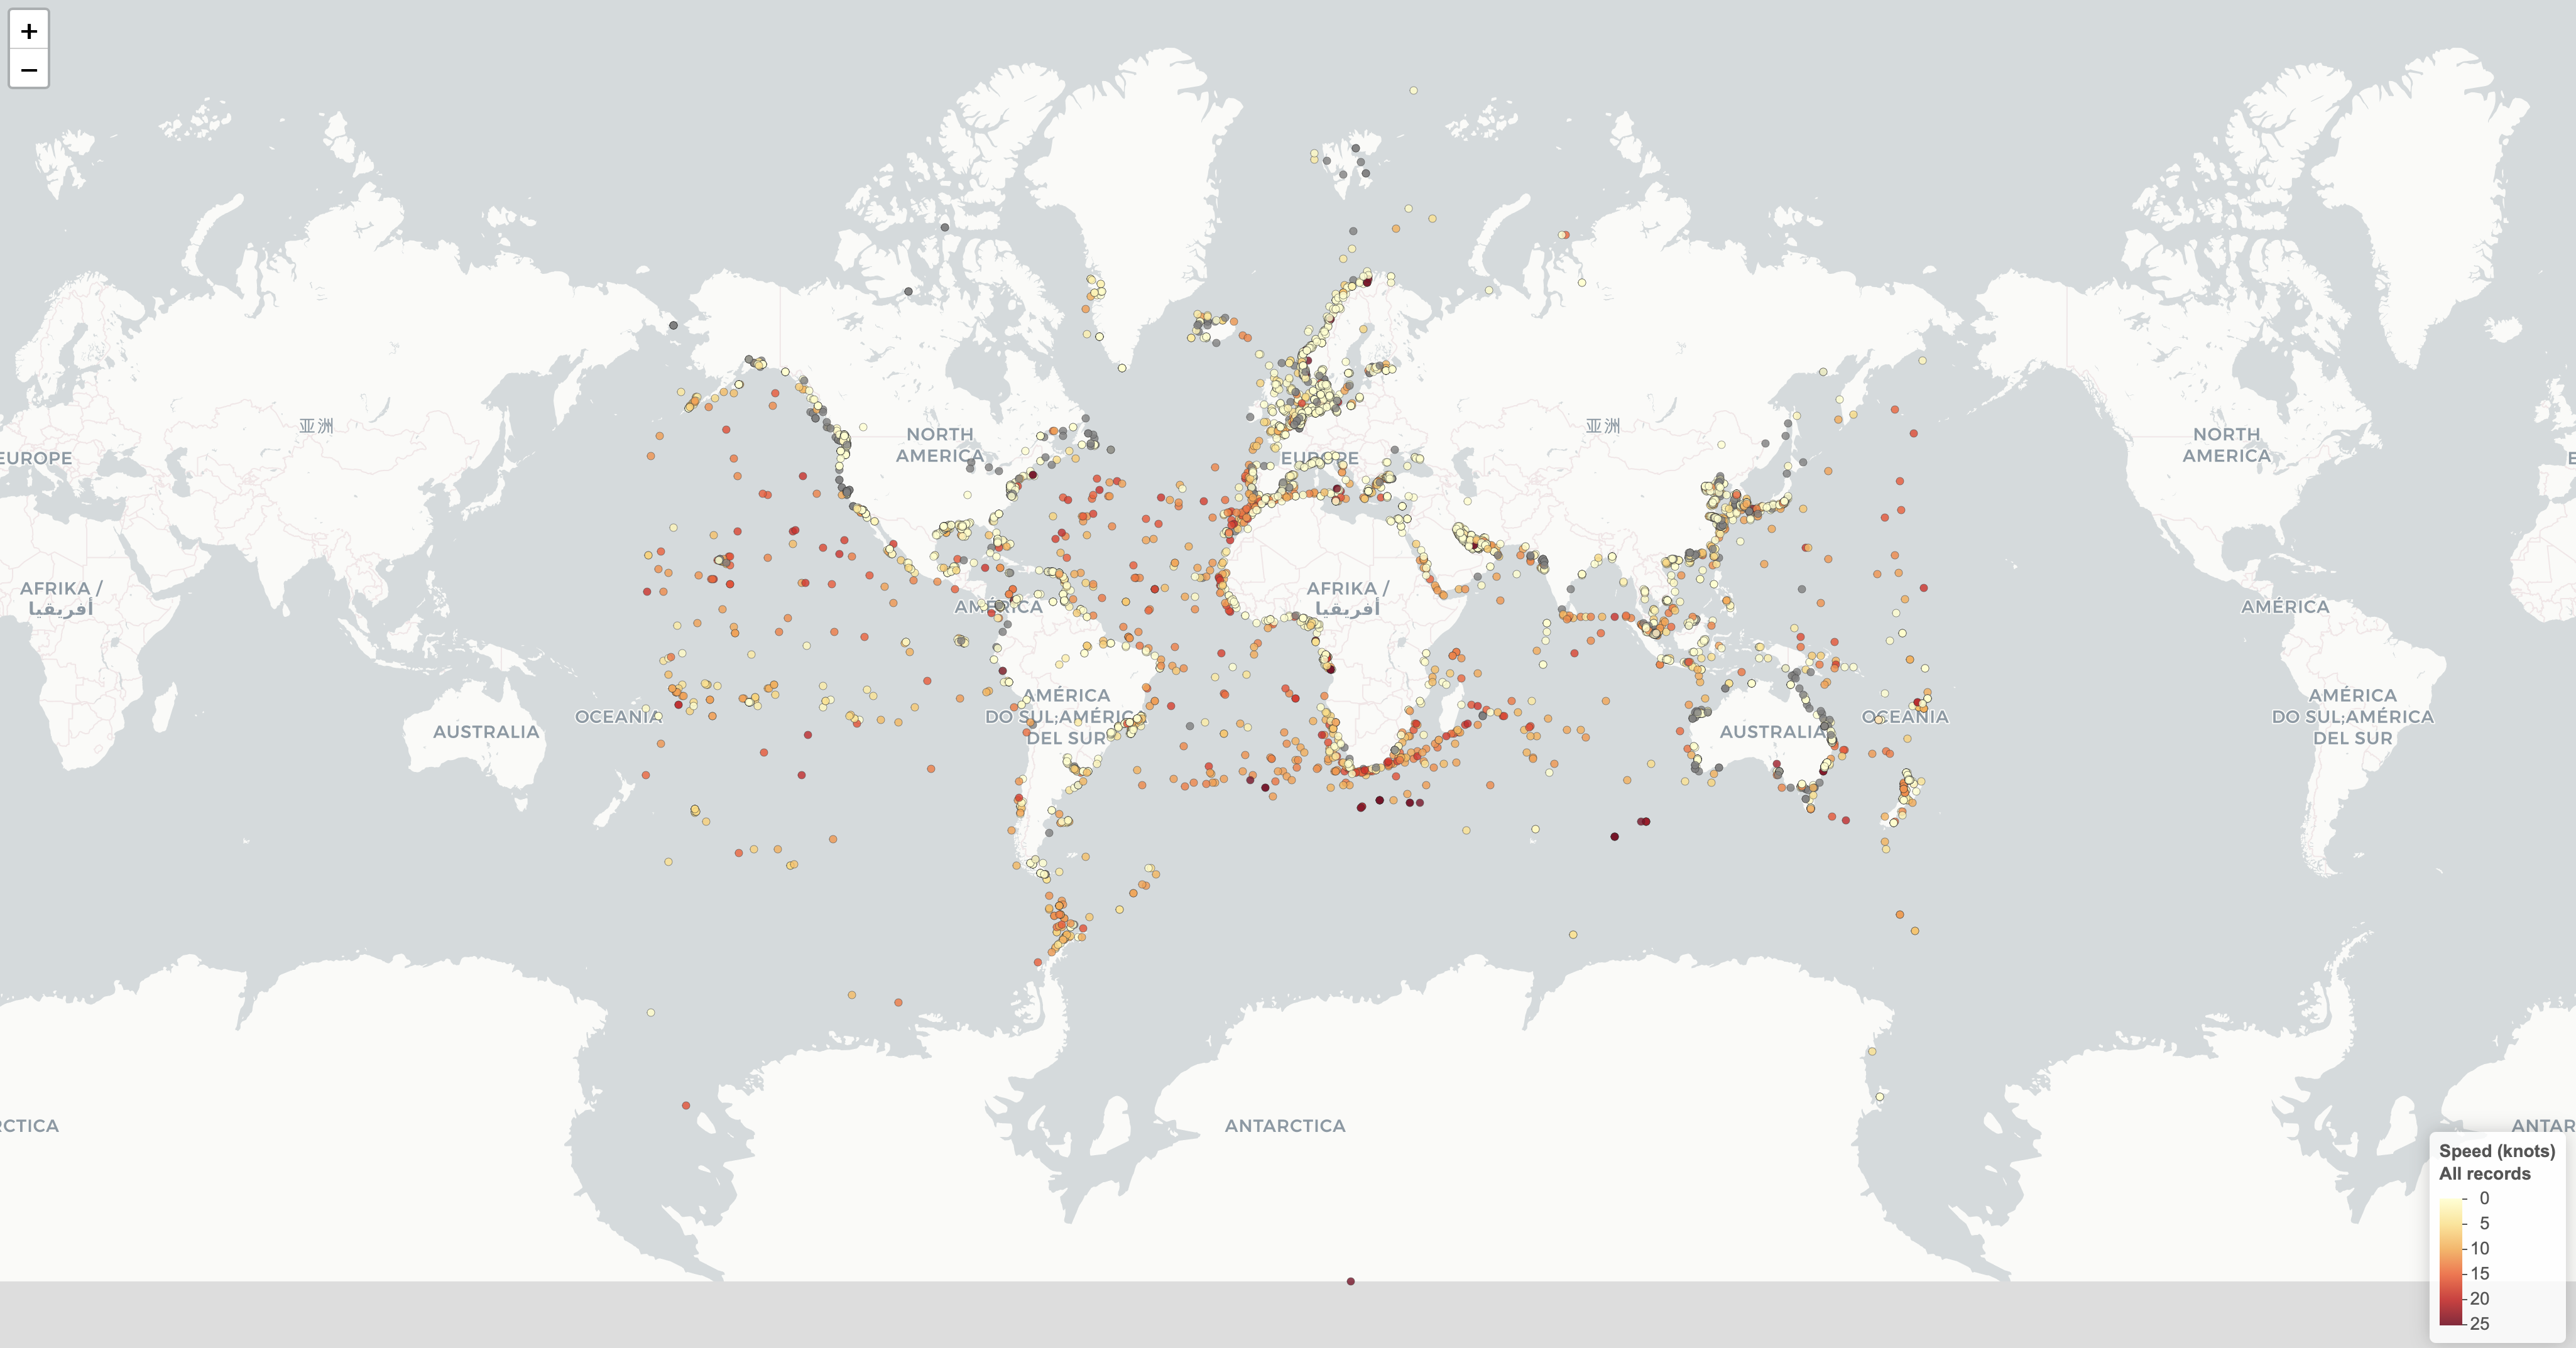
\includegraphics[width=0.9\textwidth]{sample_map_full.png}
    \caption{\textbf{Worldwide sample positions by speed.} All sampled AIS positions, coloured by speed over ground (knots, capped at 25).}
    \label{fig:map-full}
\end{figure}

A second map (Figure~\ref{fig:map-sat}) was generated using only observations
collected via satellite AIS. Compared with the full sample, the satellite-only map
appears less dense and contains noticeably fewer observations in coastal areas. This
pattern is expected: near coasts and busy ports, large numbers of vessels transmit
simultaneously, so satellites receive many overlapping messages and signal collisions
reduce the number of successfully decoded reports, whereas terrestrial receivers cover
exactly these dense coastal zones well \cite{5}. The satellite layer therefore contributes
most in open-ocean areas that lie beyond terrestrial range.

\begin{figure}[H]
    \centering
    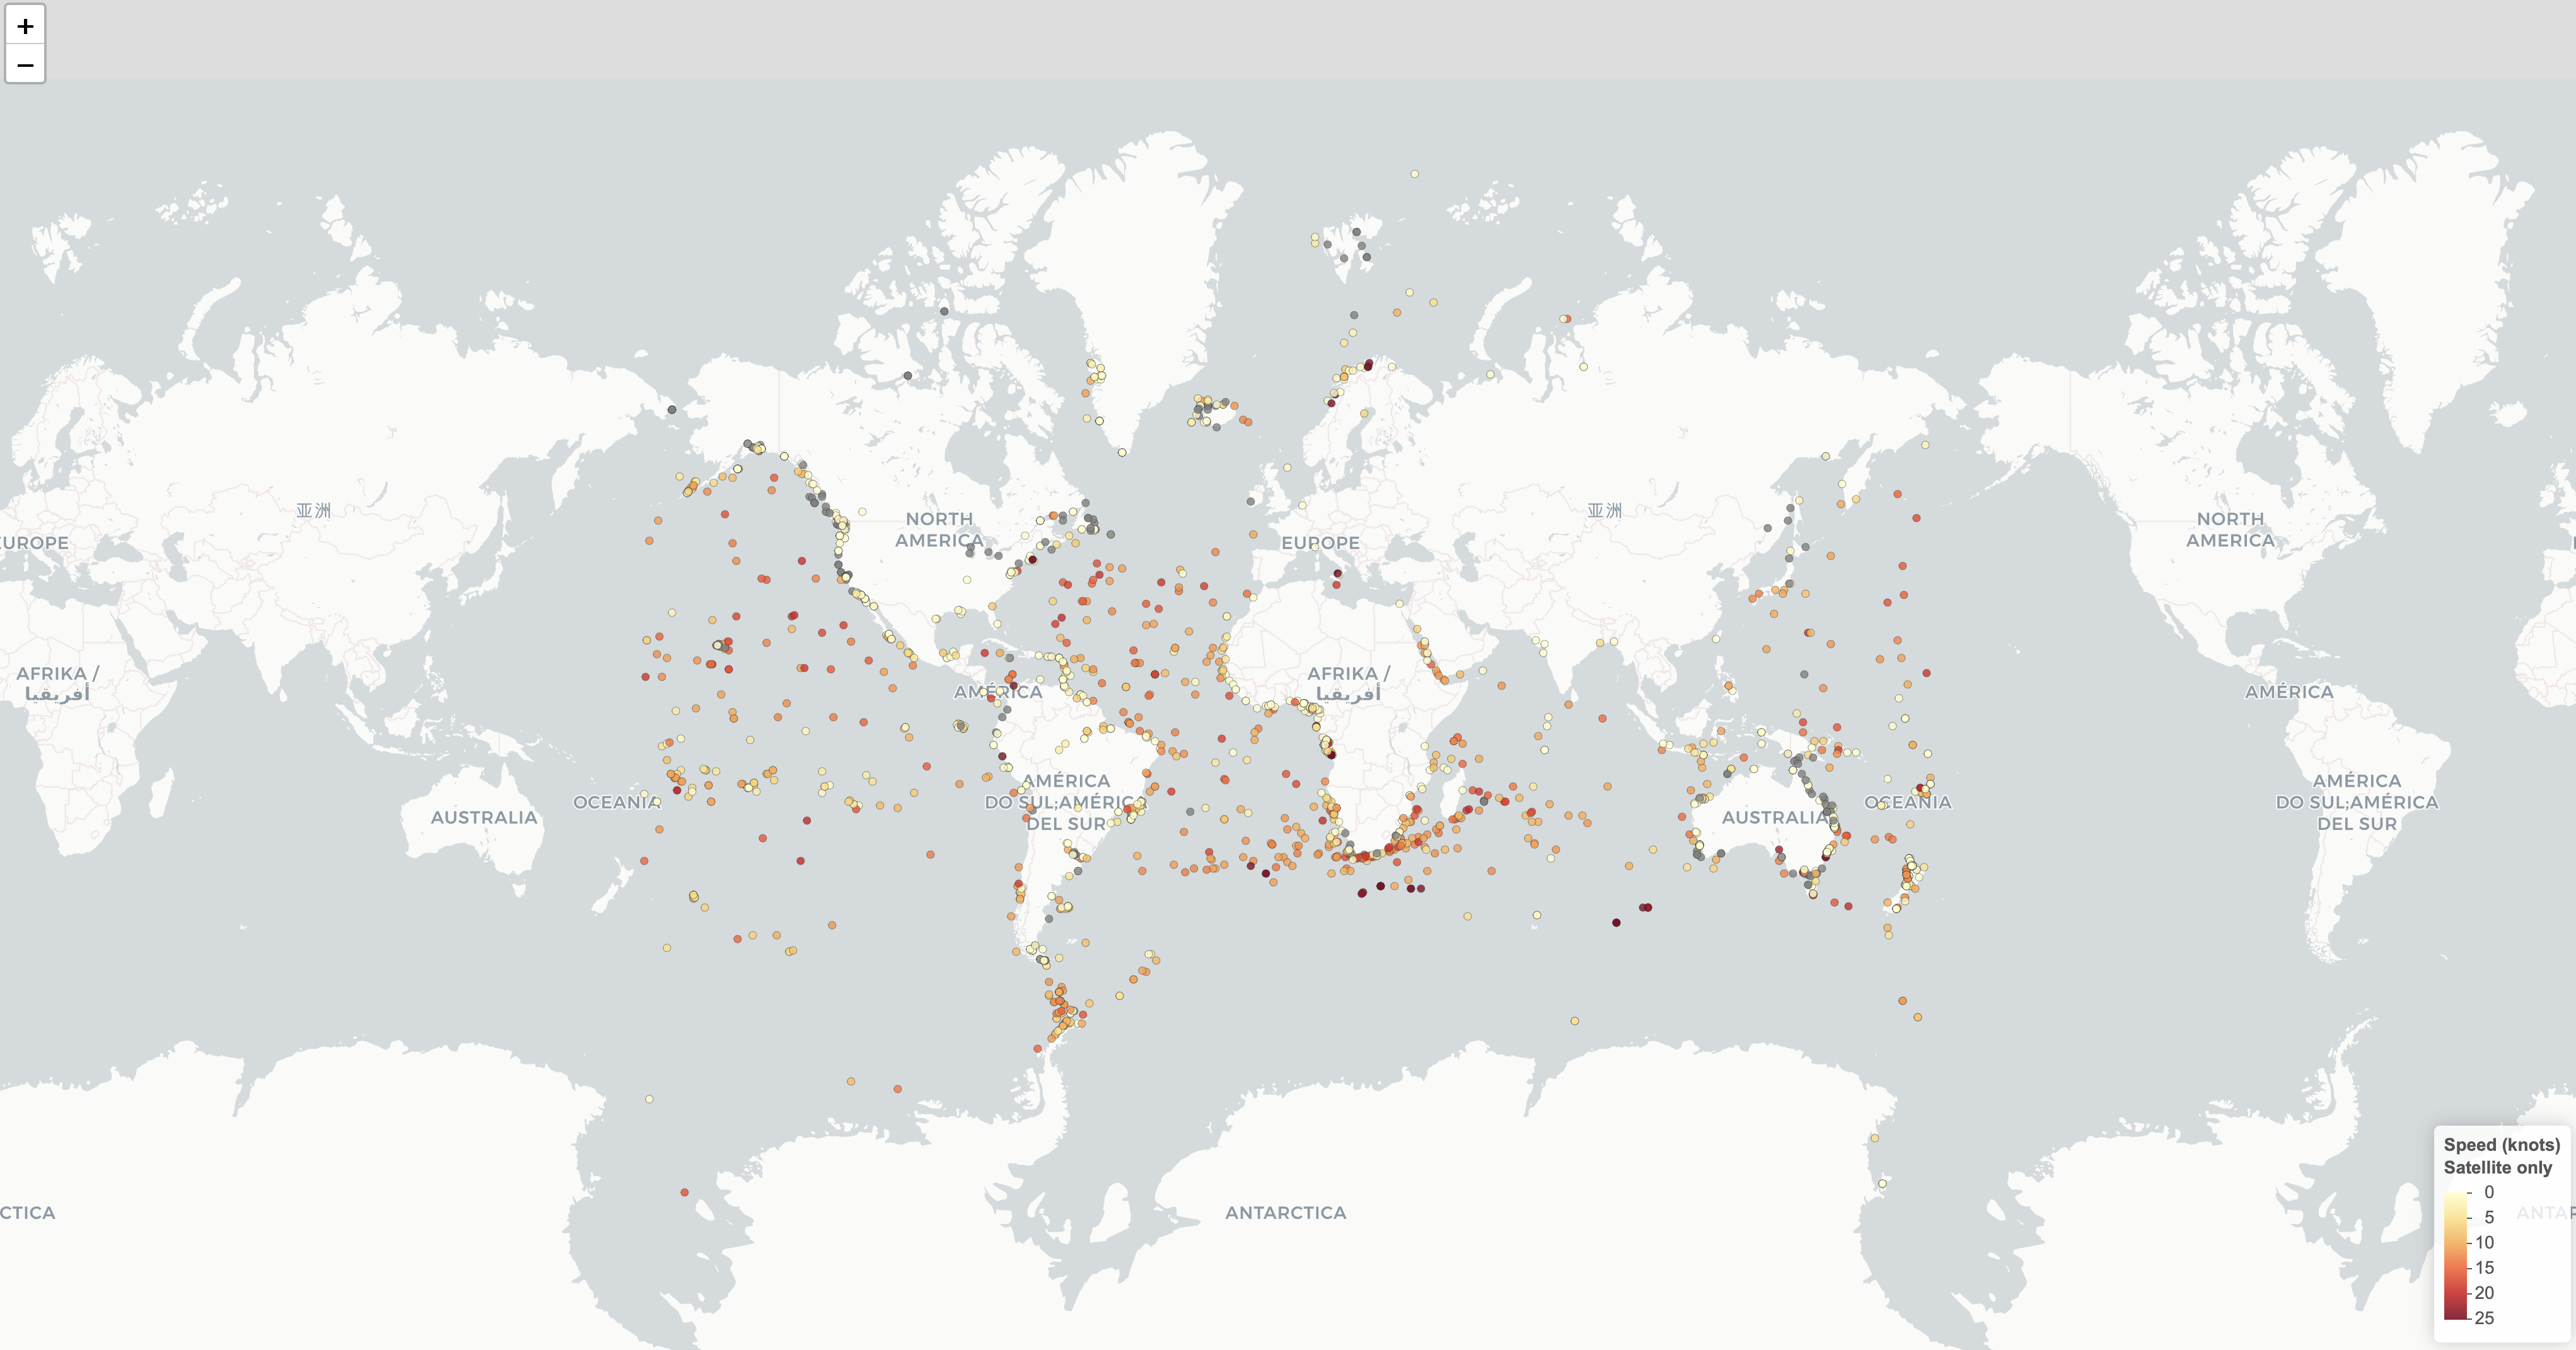
\includegraphics[width=0.9\textwidth]{sample_map_satellite.png}
    \caption{\textbf{Satellite-only sample positions.} The sampled AIS positions collected via satellite AIS, sparser near coasts than the full sample.}
    \label{fig:map-sat}
\end{figure}

% ======================================================================================
% 5.2 Individual Vessel Tracks
% ======================================================================================

\subsection {Individual Vessel Tracks}

\textbf{MMSI 2579999 --- a data-quality example.}
Querying all records for MMSI 2579999 returns 10,828 messages within a single day,
but the data are clearly not those of one physical vessel. The speed field is missing
for every record, and the 7,827 distinct positions are scattered across the entire
globe, spanning latitudes from about $-38^\circ$ to $65^\circ$ and longitudes from
about $-58^\circ$ to $148^\circ$. Consecutive messages, only seconds apart, jump
between the North Sea, south-eastern Australia, and the coast of South Korea, which
implies physically impossible speeds. Such a pattern is a textbook symptom of a shared
or default MMSI: the same identifier is transmitted by many unrelated devices, or used
as a placeholder, so that reconstructing a single track produces the characteristic
worldwide ``zigzag'' \cite{9,10}. The identifier should therefore be treated as unreliable
and excluded from movement analysis rather than interpreted as a real voyage.

\textbf{MMSI 563040400 --- a vessel at berth.}
This Singapore-flagged vessel (MMSI prefix 563) reports 4,313 records over roughly four
days (1--5 January 2021). All positions fall within a very small area around
$44.0^\circ$--$44.1^\circ$N and $28.7^\circ$--$28.8^\circ$E, which corresponds to the
Port of Constan\c{t}a on the Romanian Black Sea coast, and the speed is zero for the
large majority of records (median 0~knots, maximum 11.7~knots). The vessel is thus
essentially stationary at berth for the observed period, with only occasional slow
movements that likely reflect repositioning within the port or minor GPS noise.
Figure~\ref{fig:track563} shows the corresponding track.

\begin{figure}[H]
    \centering
    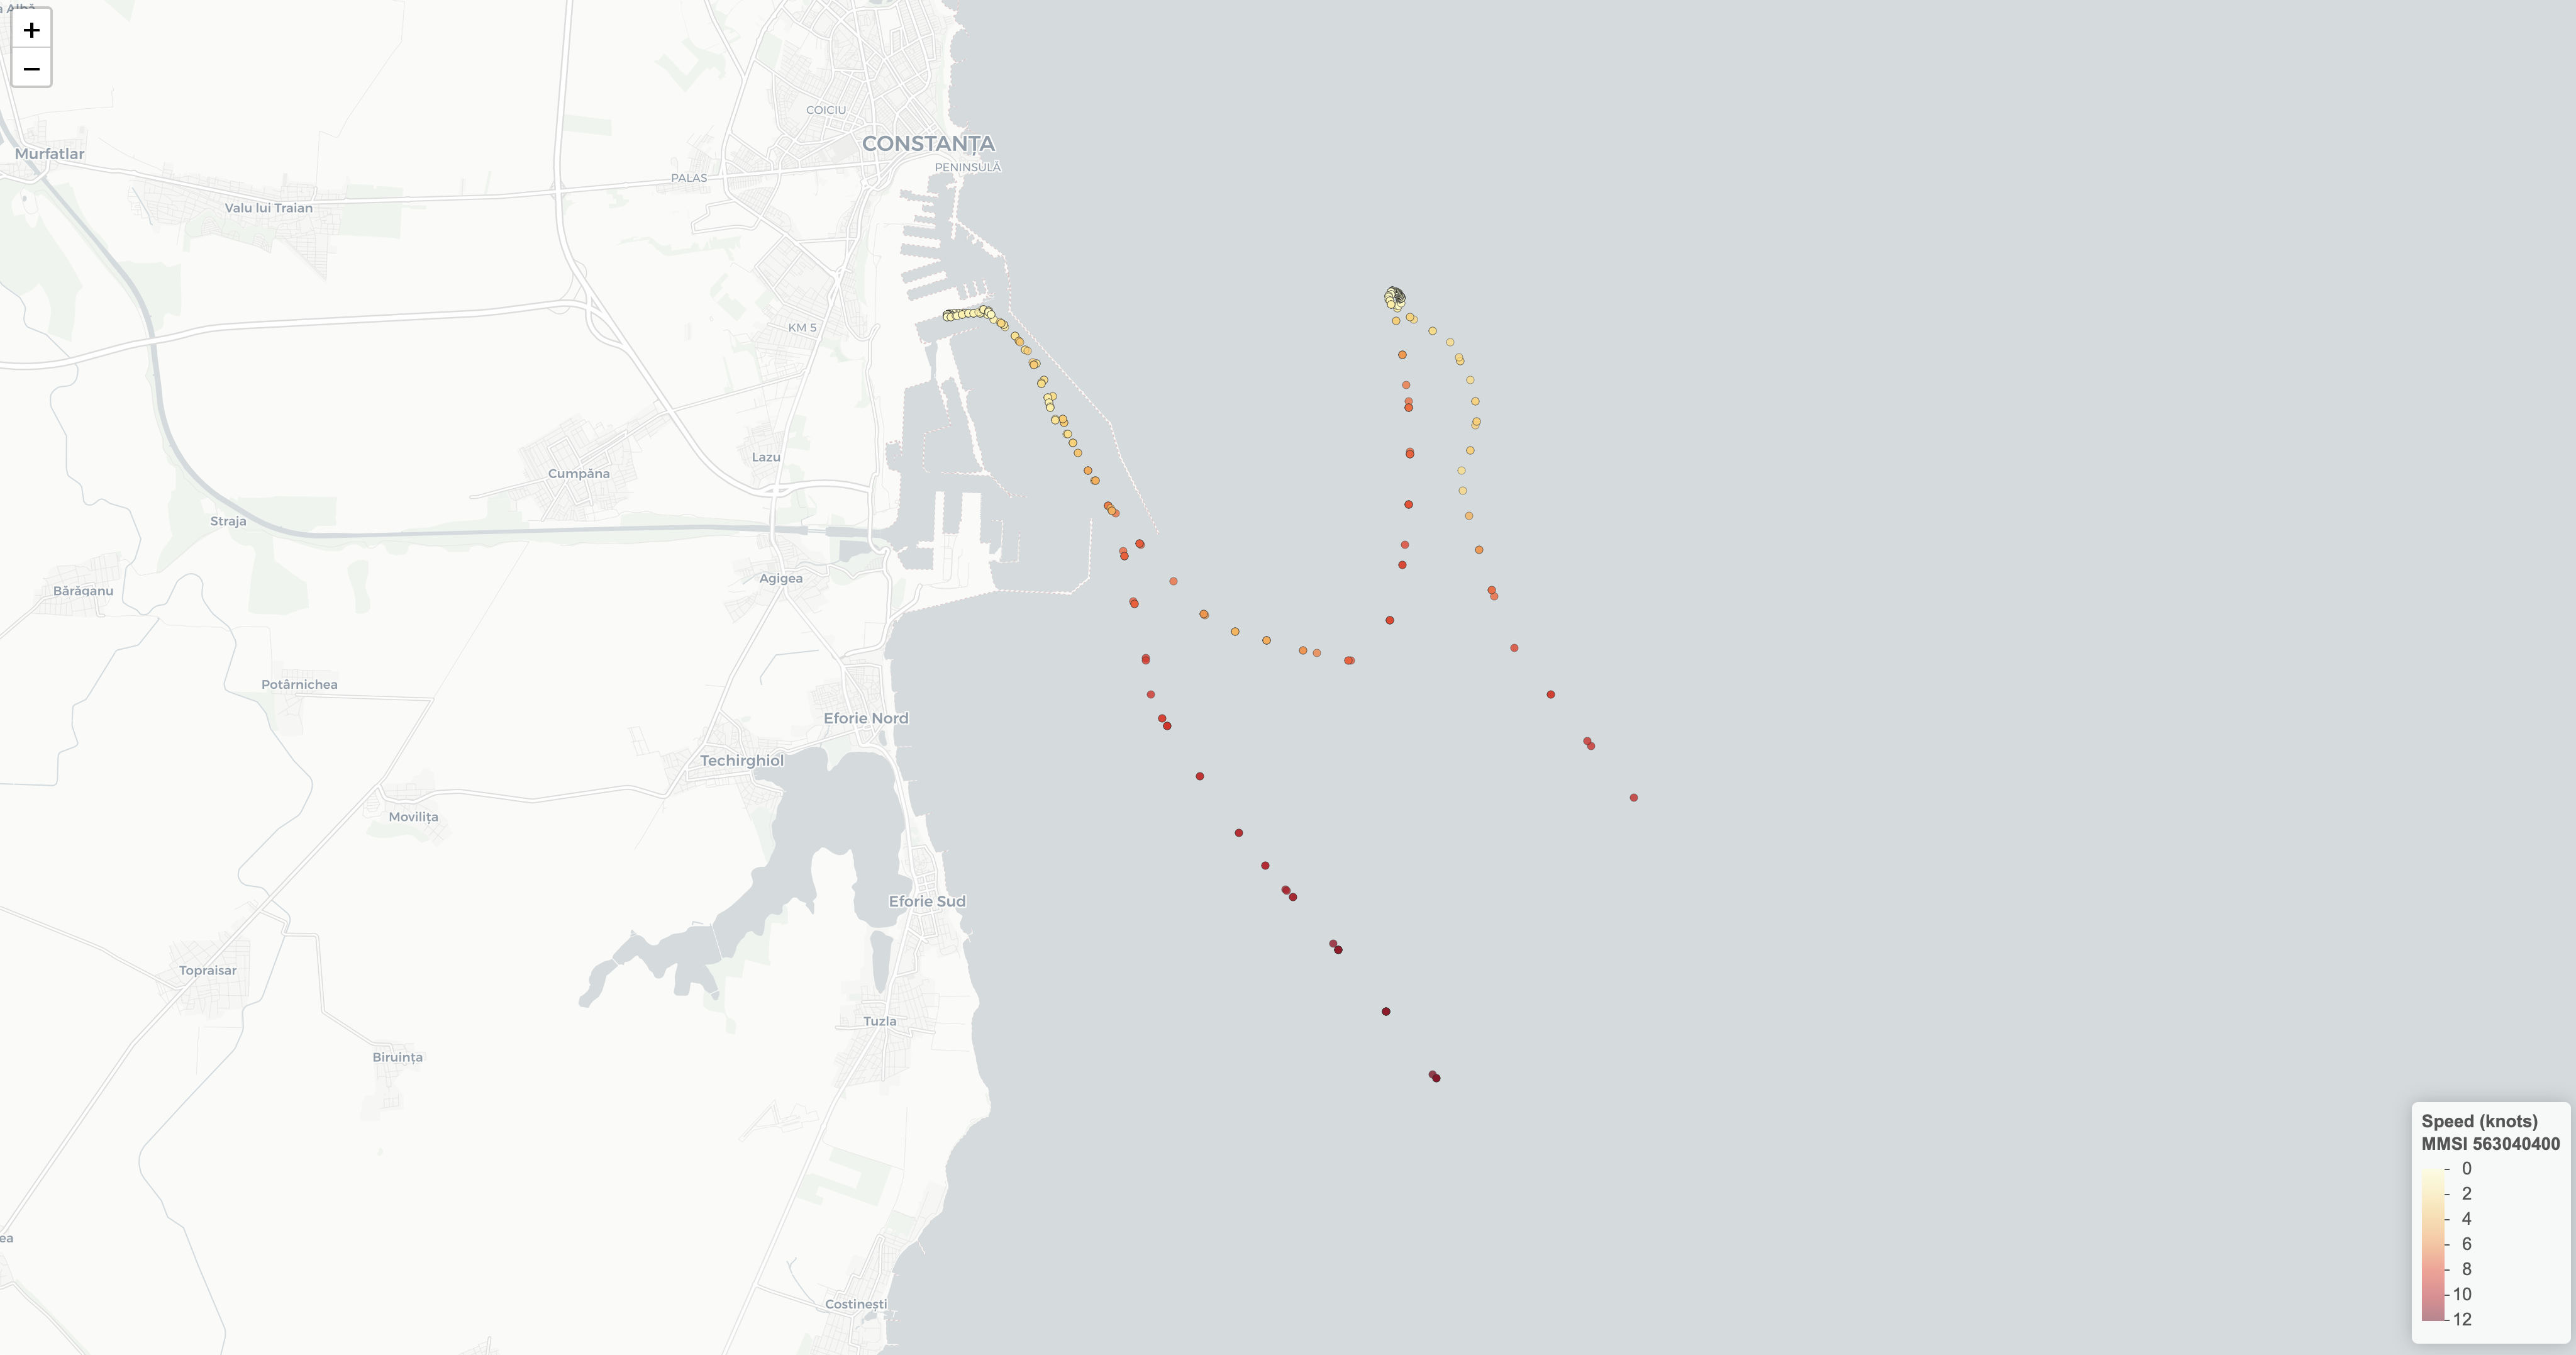
\includegraphics[width=0.75\textwidth]{track_563040400.png}
    \caption{\textbf{Track of MMSI 563040400 (Port of Constan\c{t}a).} The vessel's positions over about four days, coloured by speed (knots, capped at 12).}
    \label{fig:track563}
\end{figure}

% ======================================================================================
% 5.3 Ship-Lock Detection
% ======================================================================================

\subsection {Ship-Lock Detection}

The vessel with MMSI 211430830 (a German-flagged vessel) was analysed over the window
2021-01-17 to 2021-01-20. The retrieved track contains 574 records between 18 and 19
January and runs along the Danube from the area east of Vienna
($\approx 17.7^\circ$E) upstream to Linz ($\approx 14.3^\circ$E), at a typical river
speed of around 3--4~knots (median 3.6~knots).

Along this route the vessel passes several ship locks, where vessels are raised or
lowered to bypass dams. \emph{In AIS data, a lock passage has a characteristic
signature}: the vessel's speed drops to near zero, its position stays within a very
small area (the lock chamber, only tens of metres across) while the gates close and the
water level changes, and because the vessel lingers, a comparatively high number of AIS
messages accumulate in that small location. The passage typically lasts in the order of
15--30 minutes. Between locks, the vessel moves continuously at a few knots. In this
track, 79 of the 574 records have a speed below 1~knot, consistent with several such
stops.

This signature motivates a transparent, rule-based detection heuristic
(\texttt{lock\_detection.R}). The decision logic is:
\begin{enumerate}
    \item Sort the track chronologically by \texttt{msg\_timestamp}.
    \item Keep only \emph{near-stationary} points with speed below 1~knot as
          candidate lock points.
    \item Group consecutive candidates together, starting a new group whenever the
          time gap to the previous candidate exceeds 30~minutes \emph{or} the spatial
          jump exceeds 300~metres (great-circle / haversine distance).
    \item Discard groups that are too short to be a plausible lock passage (shorter
          than 5~minutes or fewer than 3 observations).
    \item For each remaining group, report the start time, end time, duration,
          mean position, and number of observations.
\end{enumerate}
The thresholds reflect the physical process: 1~knot separates genuine stops from
normal river travel; 300~metres keeps a group inside a single lock chamber while
tolerating GPS scatter; and the 5-minute / 3-point minimum removes brief drifts and
isolated noise. The 30-minute gap allows for sparse reporting while a vessel waits.

Applying the heuristic to the track yields the five candidate passages in
Table~\ref{tab:locks}, also shown on the map in Figure~\ref{fig:locks}, where detected
locks are marked in red along the blue trajectory. Four of the five are plausible lock
passages of 18--25 minutes spaced along the Danube between Vienna and Linz. The fifth,
lasting 132 minutes at the western end of the route ($14.35^\circ$E, Linz), is almost
certainly the vessel's final mooring at its destination rather than a lock; it is
flagged because a long stop at one location matches the same low-speed, tightly
clustered pattern.

\begin{table}[H]
\caption{\textbf{Detected ship-lock passages for MMSI 211430830.} Start, end, duration, mean position, and observation count of each candidate lock on the Danube (18--19 January 2021).}
\label{tab:locks}
\vspace{0.2cm}
\centering
\small
\begin{tabular}{@{}llrrrr@{}}
\toprule
{\bfseries Start (UTC)} & {\bfseries End (UTC)} & {\bfseries Dur.\ (min)} & {\bfseries Lat} & {\bfseries Lon} & {\bfseries Obs} \\
\midrule
2021-01-18 05:21 & 2021-01-18 05:46 &  24.5 & 47.883 & 17.541 &  6 \\
2021-01-18 19:20 & 2021-01-18 19:41 &  21.7 & 48.176 & 16.479 &  8 \\
2021-01-18 20:55 & 2021-01-18 21:18 &  23.0 & 48.244 & 16.386 & 12 \\
2021-01-19 20:45 & 2021-01-19 21:03 &  18.2 & 48.250 & 14.432 &  7 \\
2021-01-19 21:45 & 2021-01-19 23:57 & 132.6 & 48.278 & 14.349 & 45 \\
\bottomrule
\end{tabular}
\end{table}

\begin{figure}[H]
    \centering
    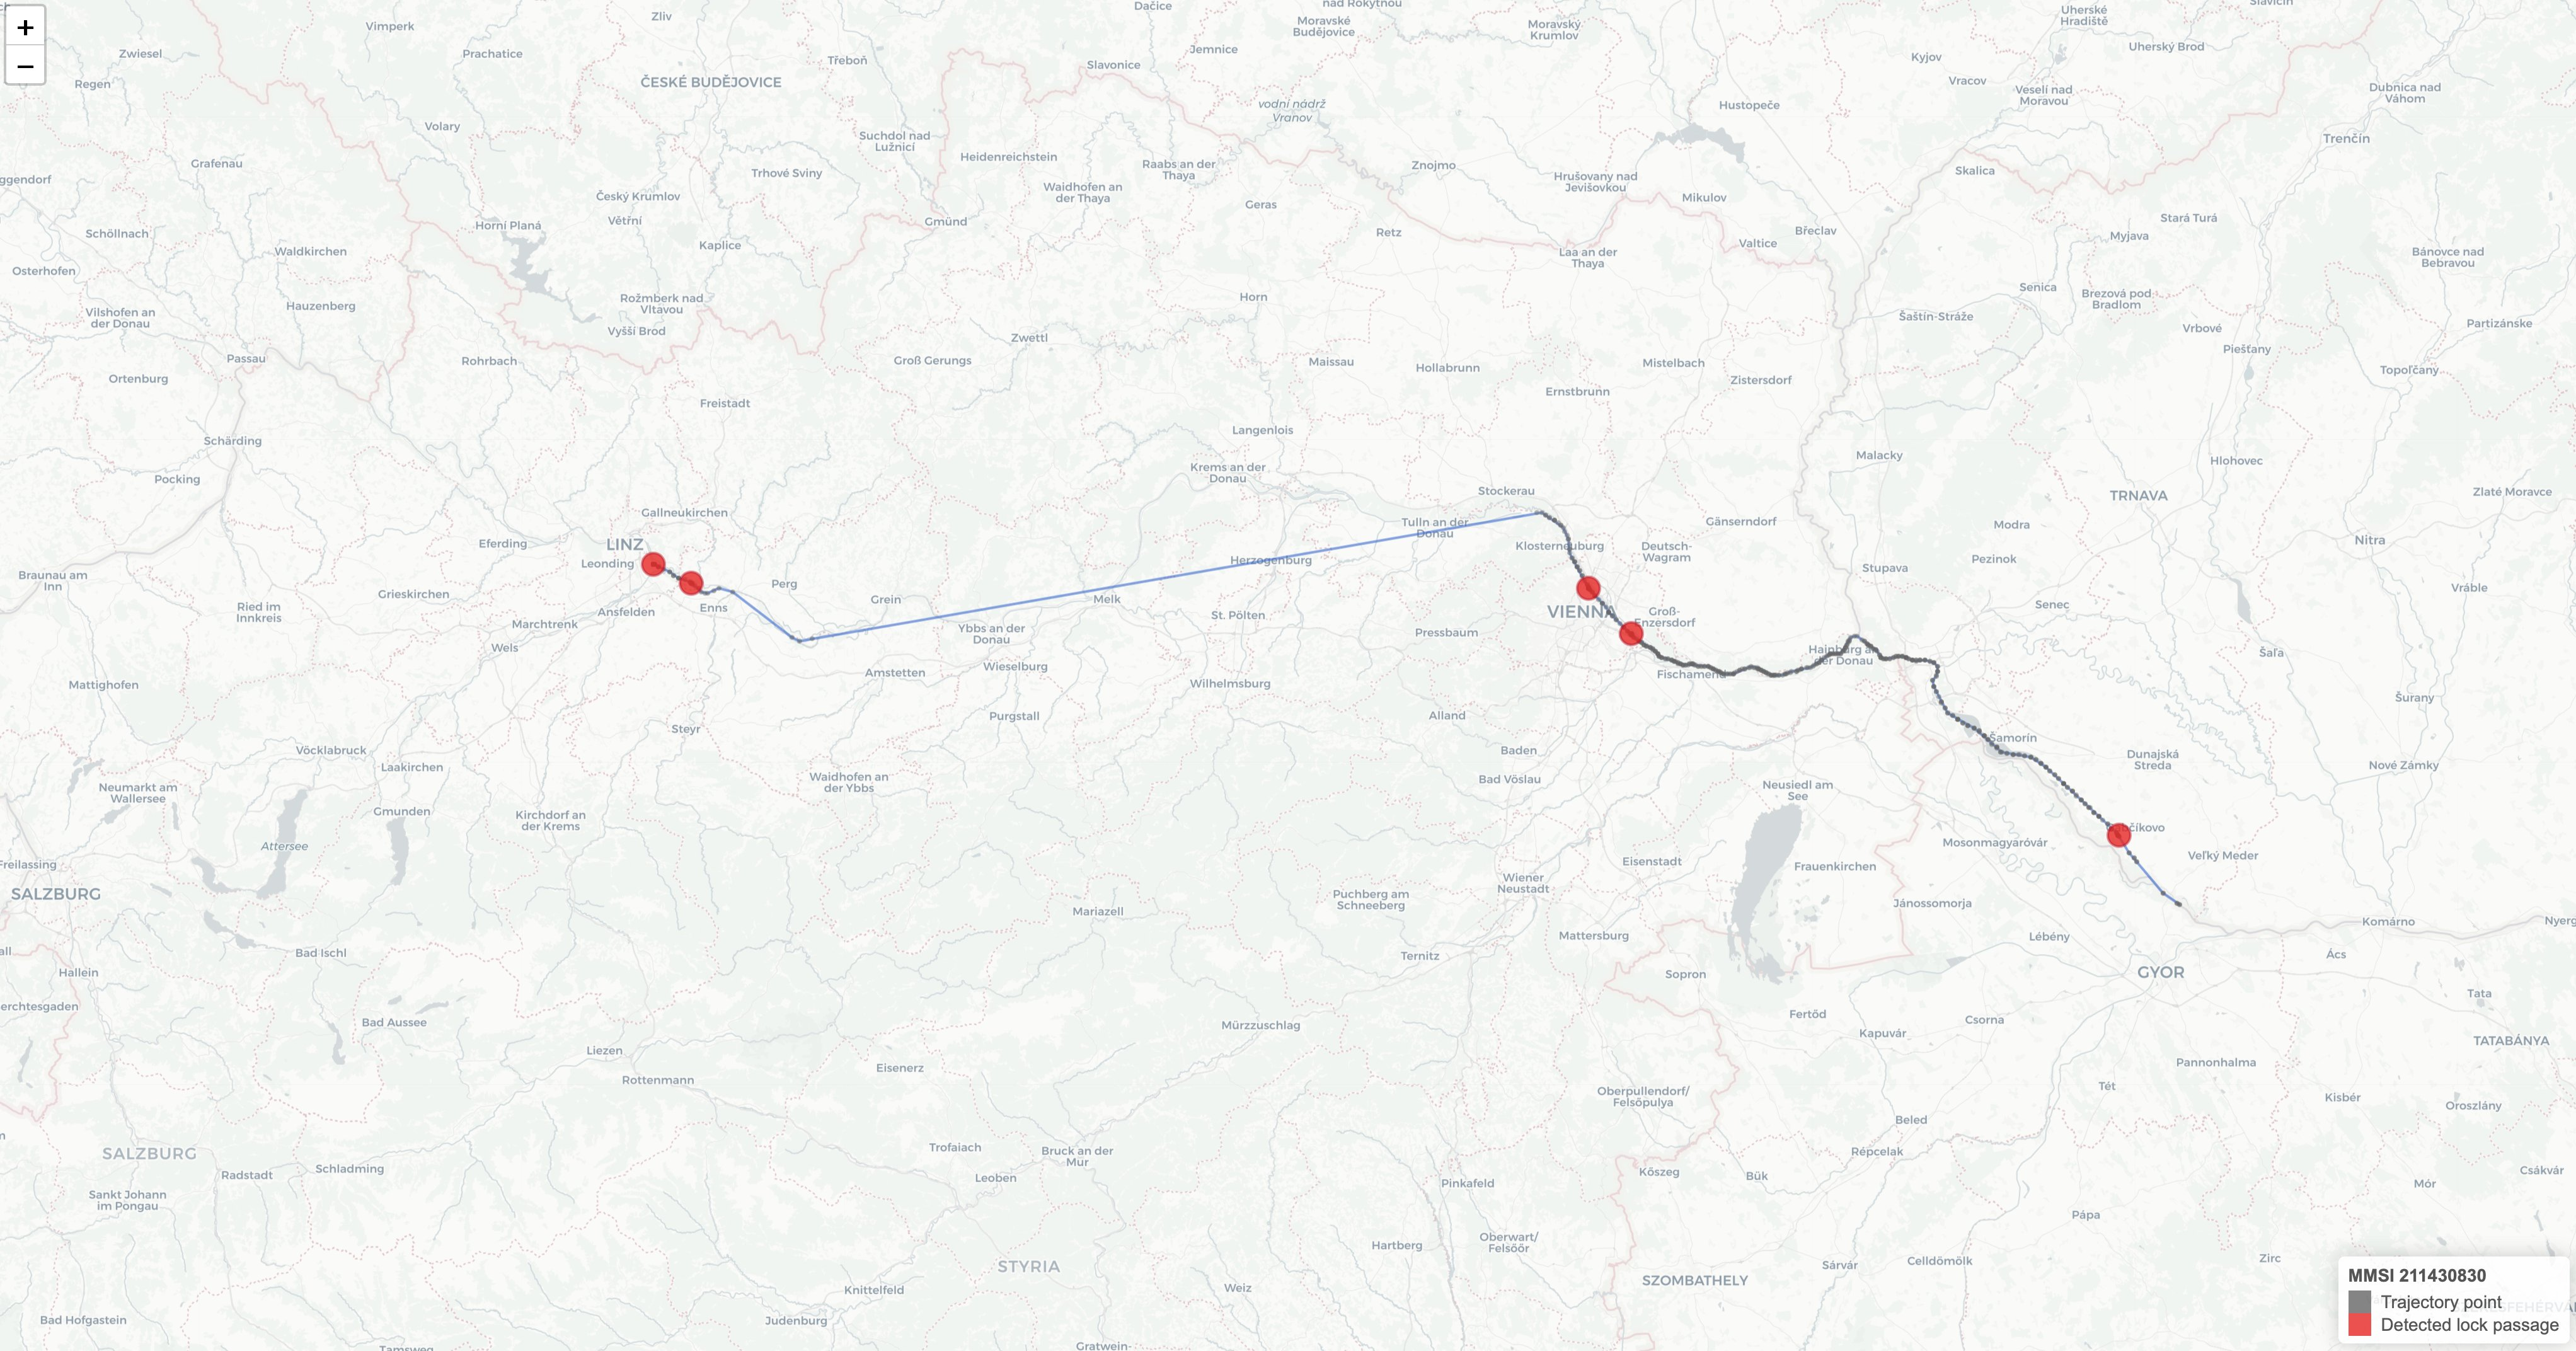
\includegraphics[width=0.9\textwidth]{track_211430830_locks.png}
    \caption{\textbf{Lock passages of MMSI 211430830.} The Danube trajectory (blue) with detected ship-lock passages highlighted in red.}
    \label{fig:locks}
\end{figure}

The goal of this heuristic is transparency and reproducibility rather than perfect
recall. Its limitations follow directly from the rules: a long stop that is not a lock
(such as the final mooring above) is reported as a false positive, while a lock taken
without dropping below 1~knot, or with very sparse reporting, could be missed. The
fixed thresholds are also tuned to inland navigation and would need adjustment for
other vessel classes. A natural improvement would replace the manual thresholds with an
\emph{unsupervised} approach: rather than hand-labelled training data, a density-based
clustering method such as DBSCAN could be applied to the low-speed points in
space and time, letting the data define the clusters and adapting automatically to
different reporting rates and lock geometries.

% ======================================================================================
% 6. AIS Traffic Density on German Rivers
% ======================================================================================

\section {AIS Traffic Density on German Rivers}

Building on the dynamic AIS records, this section combines vessel positions with
geographic information about German rivers to analyse how traffic is distributed
across the inland waterway network. The analysis is based on the
\texttt{ais\_germany} table, which contains AIS records for vessels tracked within
Germany, and uses the H3 spatial indexing system to assign each record to a river.

% ======================================================================================
% 6.1 River Geometries and Study Data
% ======================================================================================

\subsection{River Geometries and Study Data}

River geometries for Germany were obtained from the \texttt{rnaturalearth} package,
which provides global river centre-lines as line geometries. The raw layer required
cleaning before it could be used. River features were first clipped to the German
national boundary, and empty or unnamed fragments were removed. The same river
sometimes appears under different language spellings; the German, English, and French
forms of the Rhine (\emph{Rhein}, \emph{Rhine}, \emph{Rhin}) were therefore merged
into a single feature, and multi-part segments of each river were dissolved into one
geometry per river. Finally, rivers with a negligible length inside Germany were
dropped: the Warta, for example, is almost entirely Polish and reduces to a sliver
of about ten metres after clipping, so it does not represent meaningful German
inland traffic. This cleaning leaves nine major rivers: the Danube (\emph{Donau}),
Elbe, Ems, Inn, Main, Mosel, Oder, Rhine, and Weser.

Because only nine rivers remain, each can be shown in its own colour with a fully
readable legend, so no further reduction to a subset of major rivers was necessary.
Figure~\ref{fig:rivers} maps the cleaned geometries over the German boundary.

\begin{figure}[H]
    \centering
    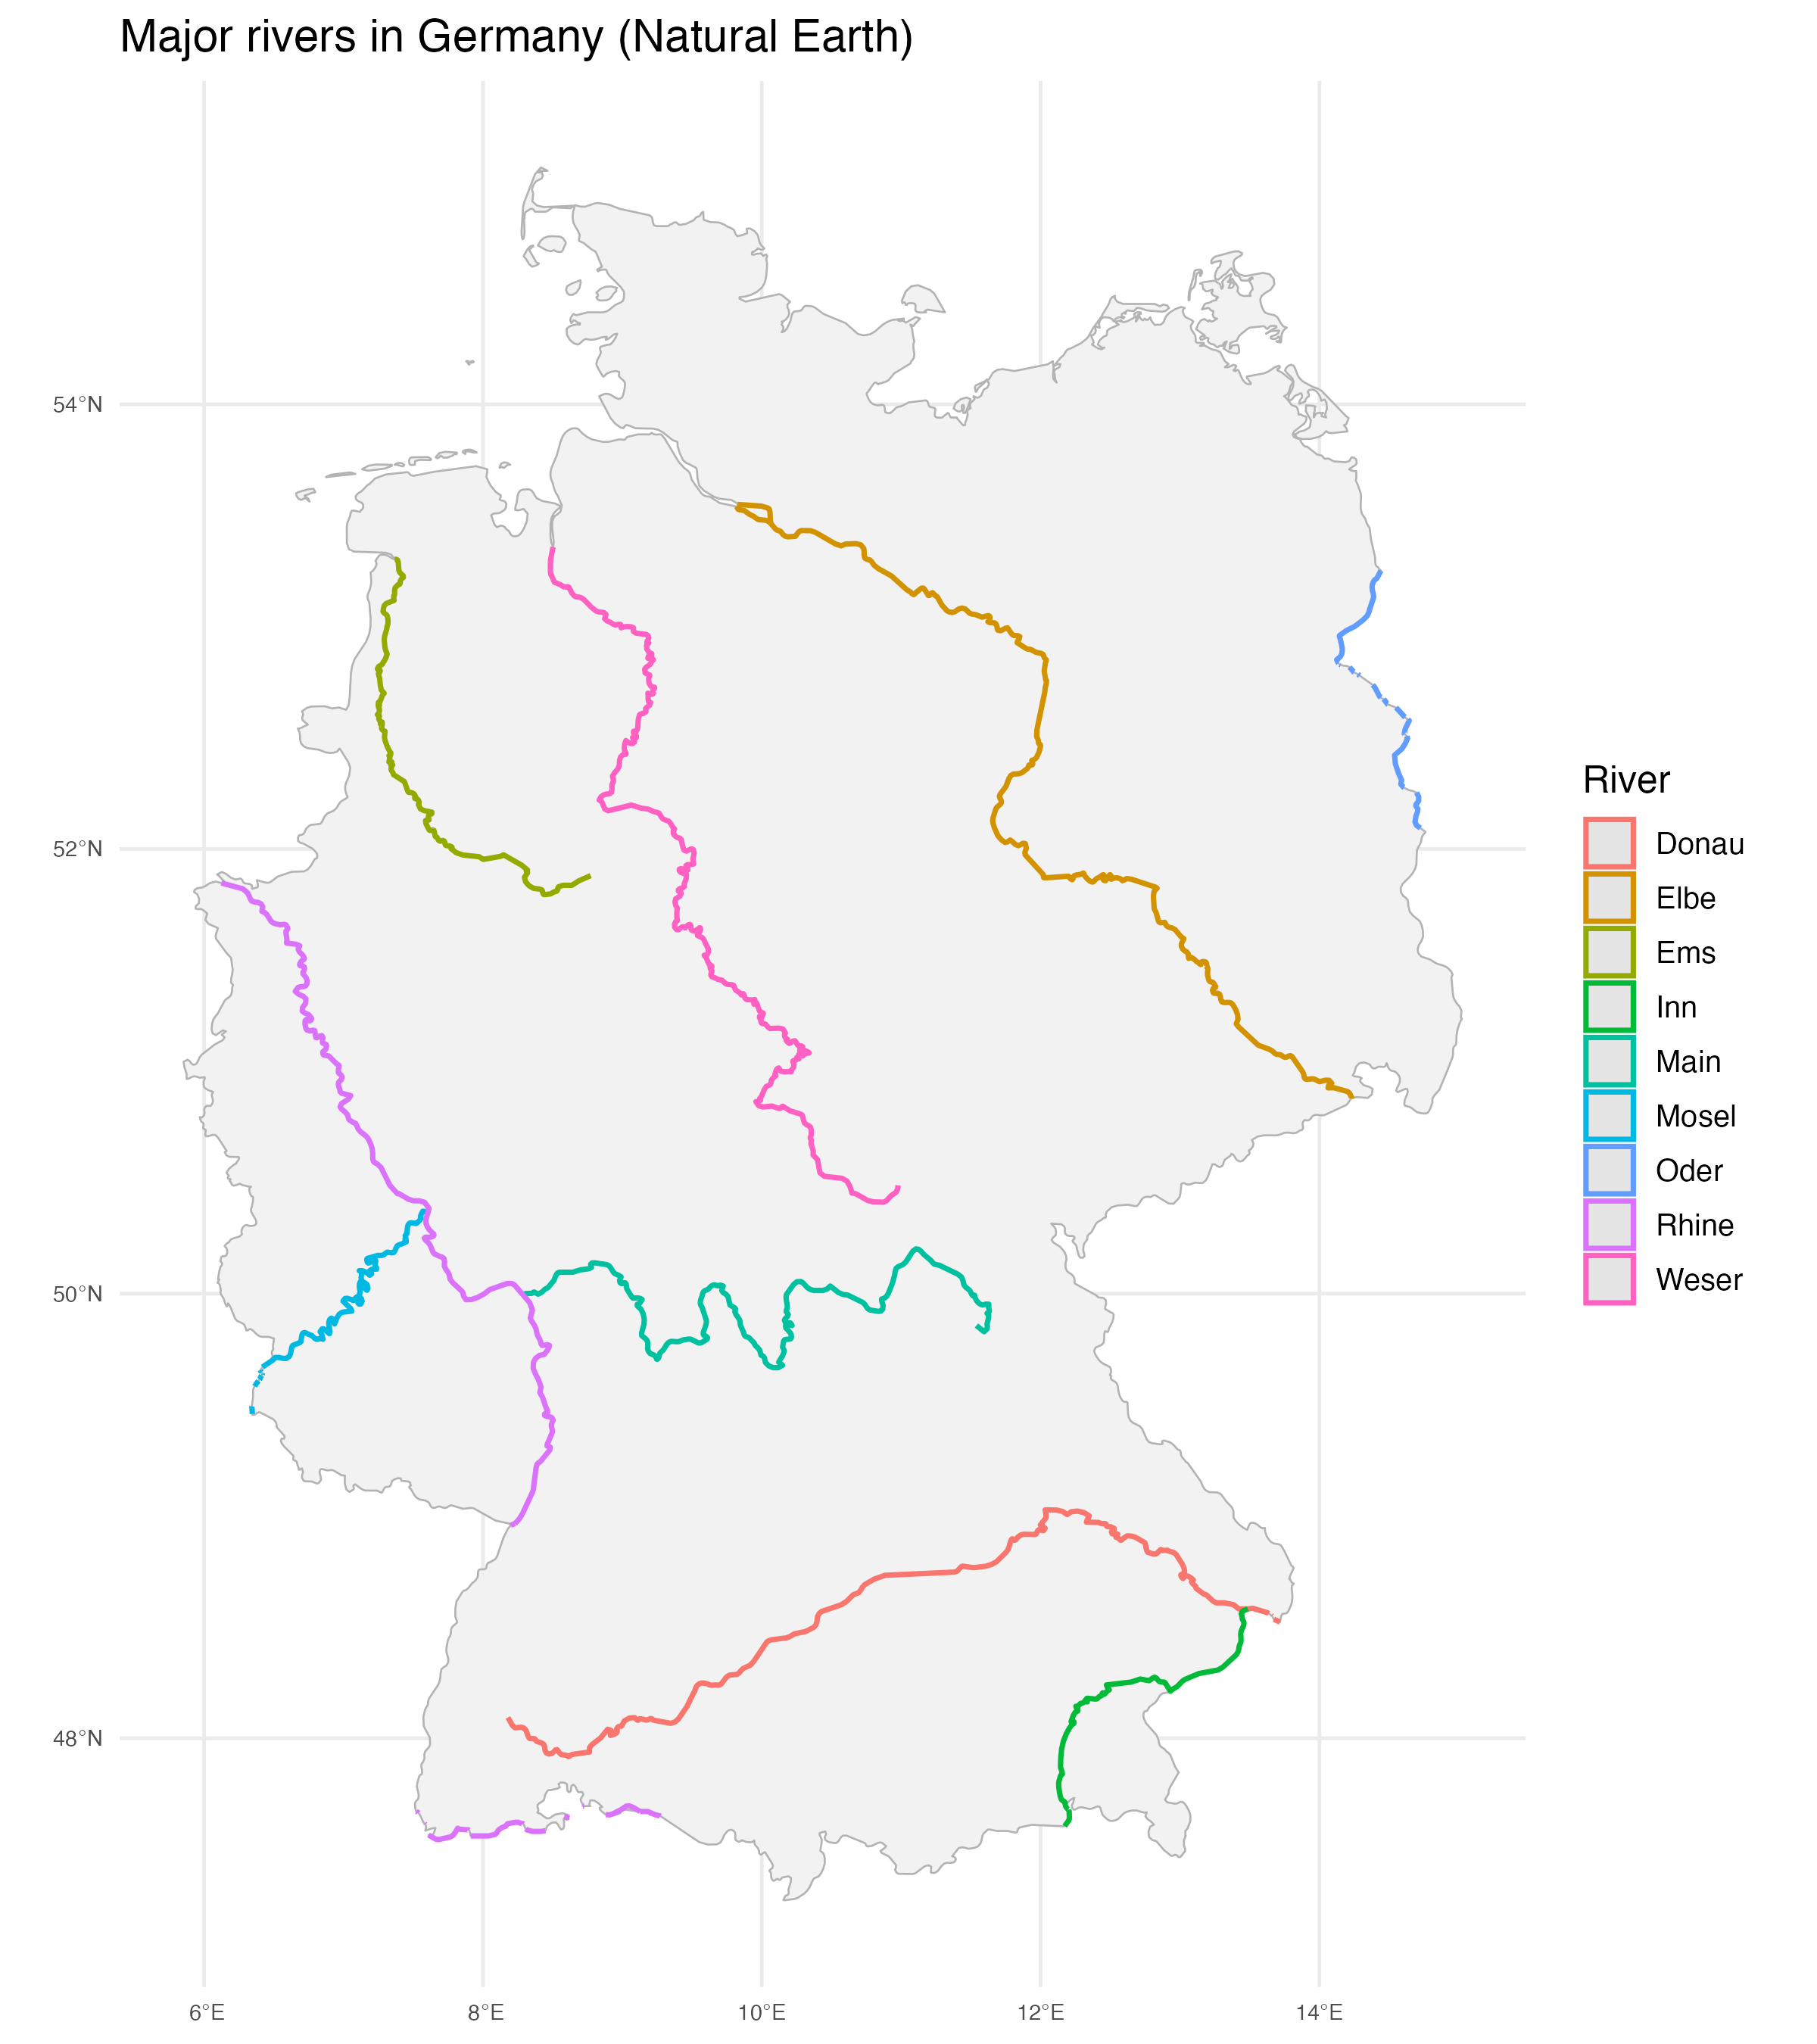
\includegraphics[width=0.55\textwidth]{german_rivers.png}
    \caption{\textbf{German river geometries.} The nine cleaned rivers, each shown in a distinct colour (Natural Earth).}
    \label{fig:rivers}
\end{figure}

The \texttt{ais\_germany} table was then queried for all tracking records on
2022-04-23, using a timestamp filter that returns only records with a message
timestamp on that date. This yields 497,990 AIS records, which form the basis for
the spatial matching below.

% ======================================================================================
% 6.2 Spatial Matching with H3
% ======================================================================================

\subsection{Spatial Matching with H3}

Determining which records lie on a river is a spatial-join problem. A naive solution
would test every AIS point against every river geometry, either by point-in-polygon
checks or by computing the distance from each point to every river segment. With
roughly half a million points and nine multi-part geometries, this scales as the
product of the two and becomes computationally expensive. The H3 indexing system
avoids this cost. H3 divides the world into a hierarchical grid of hexagonal cells,
each identified by a unique integer index, with the resolution controlling cell size
(coarse continent-scale cells at low resolutions, fine metre-scale cells at high
ones) \cite{13}. Converting a coordinate to its H3 index reduces the spatial-join to a
key lookup: each cell index acts as a key in a hash table, a structure that maps keys
to values with average constant-time retrieval. Instead of comparing geometries, the
analysis only has to check whether a point's cell index appears in the set of cell
indices covered by the rivers, which turns an expensive geometric comparison into a
fast set membership test that scales linearly with the number of points. Hexagonal
cells additionally have uniform adjacency, since every neighbour shares an edge at an
equal centre-to-centre distance, which makes them better suited to distance-based
reasoning than square grids.

Following the task specification, H3 resolution~7 was used, where a cell spans
roughly 1.2~km. Each AIS record was converted to its H3 cell from its latitude and
longitude. The rivers, however, are line geometries and cannot be filled with cells
directly, so each river line was buffered into a thin corridor before being converted
to cells. A buffer of 750~m (a corridor about 1.5~km wide) was chosen because it is
slightly wider than one resolution-7 cell: this keeps each river at least one cell
wide along its whole length and absorbs the offset between a vessel's reported
position and the mapped river centre-line, while remaining narrow enough not to
absorb large amounts of nearby non-river traffic. Buffering was performed in a metric
projection (UTM~32N) so that the distance is expressed in true metres. This produced
1,168 unique river cells in total.

Matching the records to rivers reduces to checking each record's cell against this
set. Where a single cell was claimed by more than one river, typically at confluences
such as the Rhine/Main or Rhine/Mosel junctions, a deterministic rule was applied:
the cell is assigned to the larger river, measured by its total number of cells. Only
two cells were affected, so the specific tie-break has no material effect on the
results, but the rule is documented for reproducibility.

% ======================================================================================
% 6.3 Traffic Distribution Results
% ======================================================================================

\subsection{Traffic Distribution Results}

Of the 497,990 records on 2022-04-23, 183,408 (36.8\%) fall on a German river, while
314,582 (63.2\%) were recorded elsewhere, such as coastal or open-water areas. A clear
majority of German AIS traffic on this date therefore occurs outside the inland river
network, which is consistent with the dominance of coastal and maritime shipping in
the dataset.

The composition of traffic also differs between the two groups. Figure~\ref{fig:rivertype}
compares the ship-type distribution on rivers and elsewhere. Off-river traffic is
dominated by Cargo vessels (29.3\%), followed by Passenger Ships (20.6\%) and Tankers
(9.2\%). On rivers, the share of Cargo drops to 19.0\% while Passenger Ships make up a
comparable 19.4\%, reflecting the role of ferries and excursion vessels on inland
waterways. Records without a reported ship type are the single largest group in both
cases and are especially prominent on rivers (46.8\%), which is consistent with a
higher presence of smaller inland craft that more often transmit incomplete static
information.

\begin{figure}[H]
    \centering
    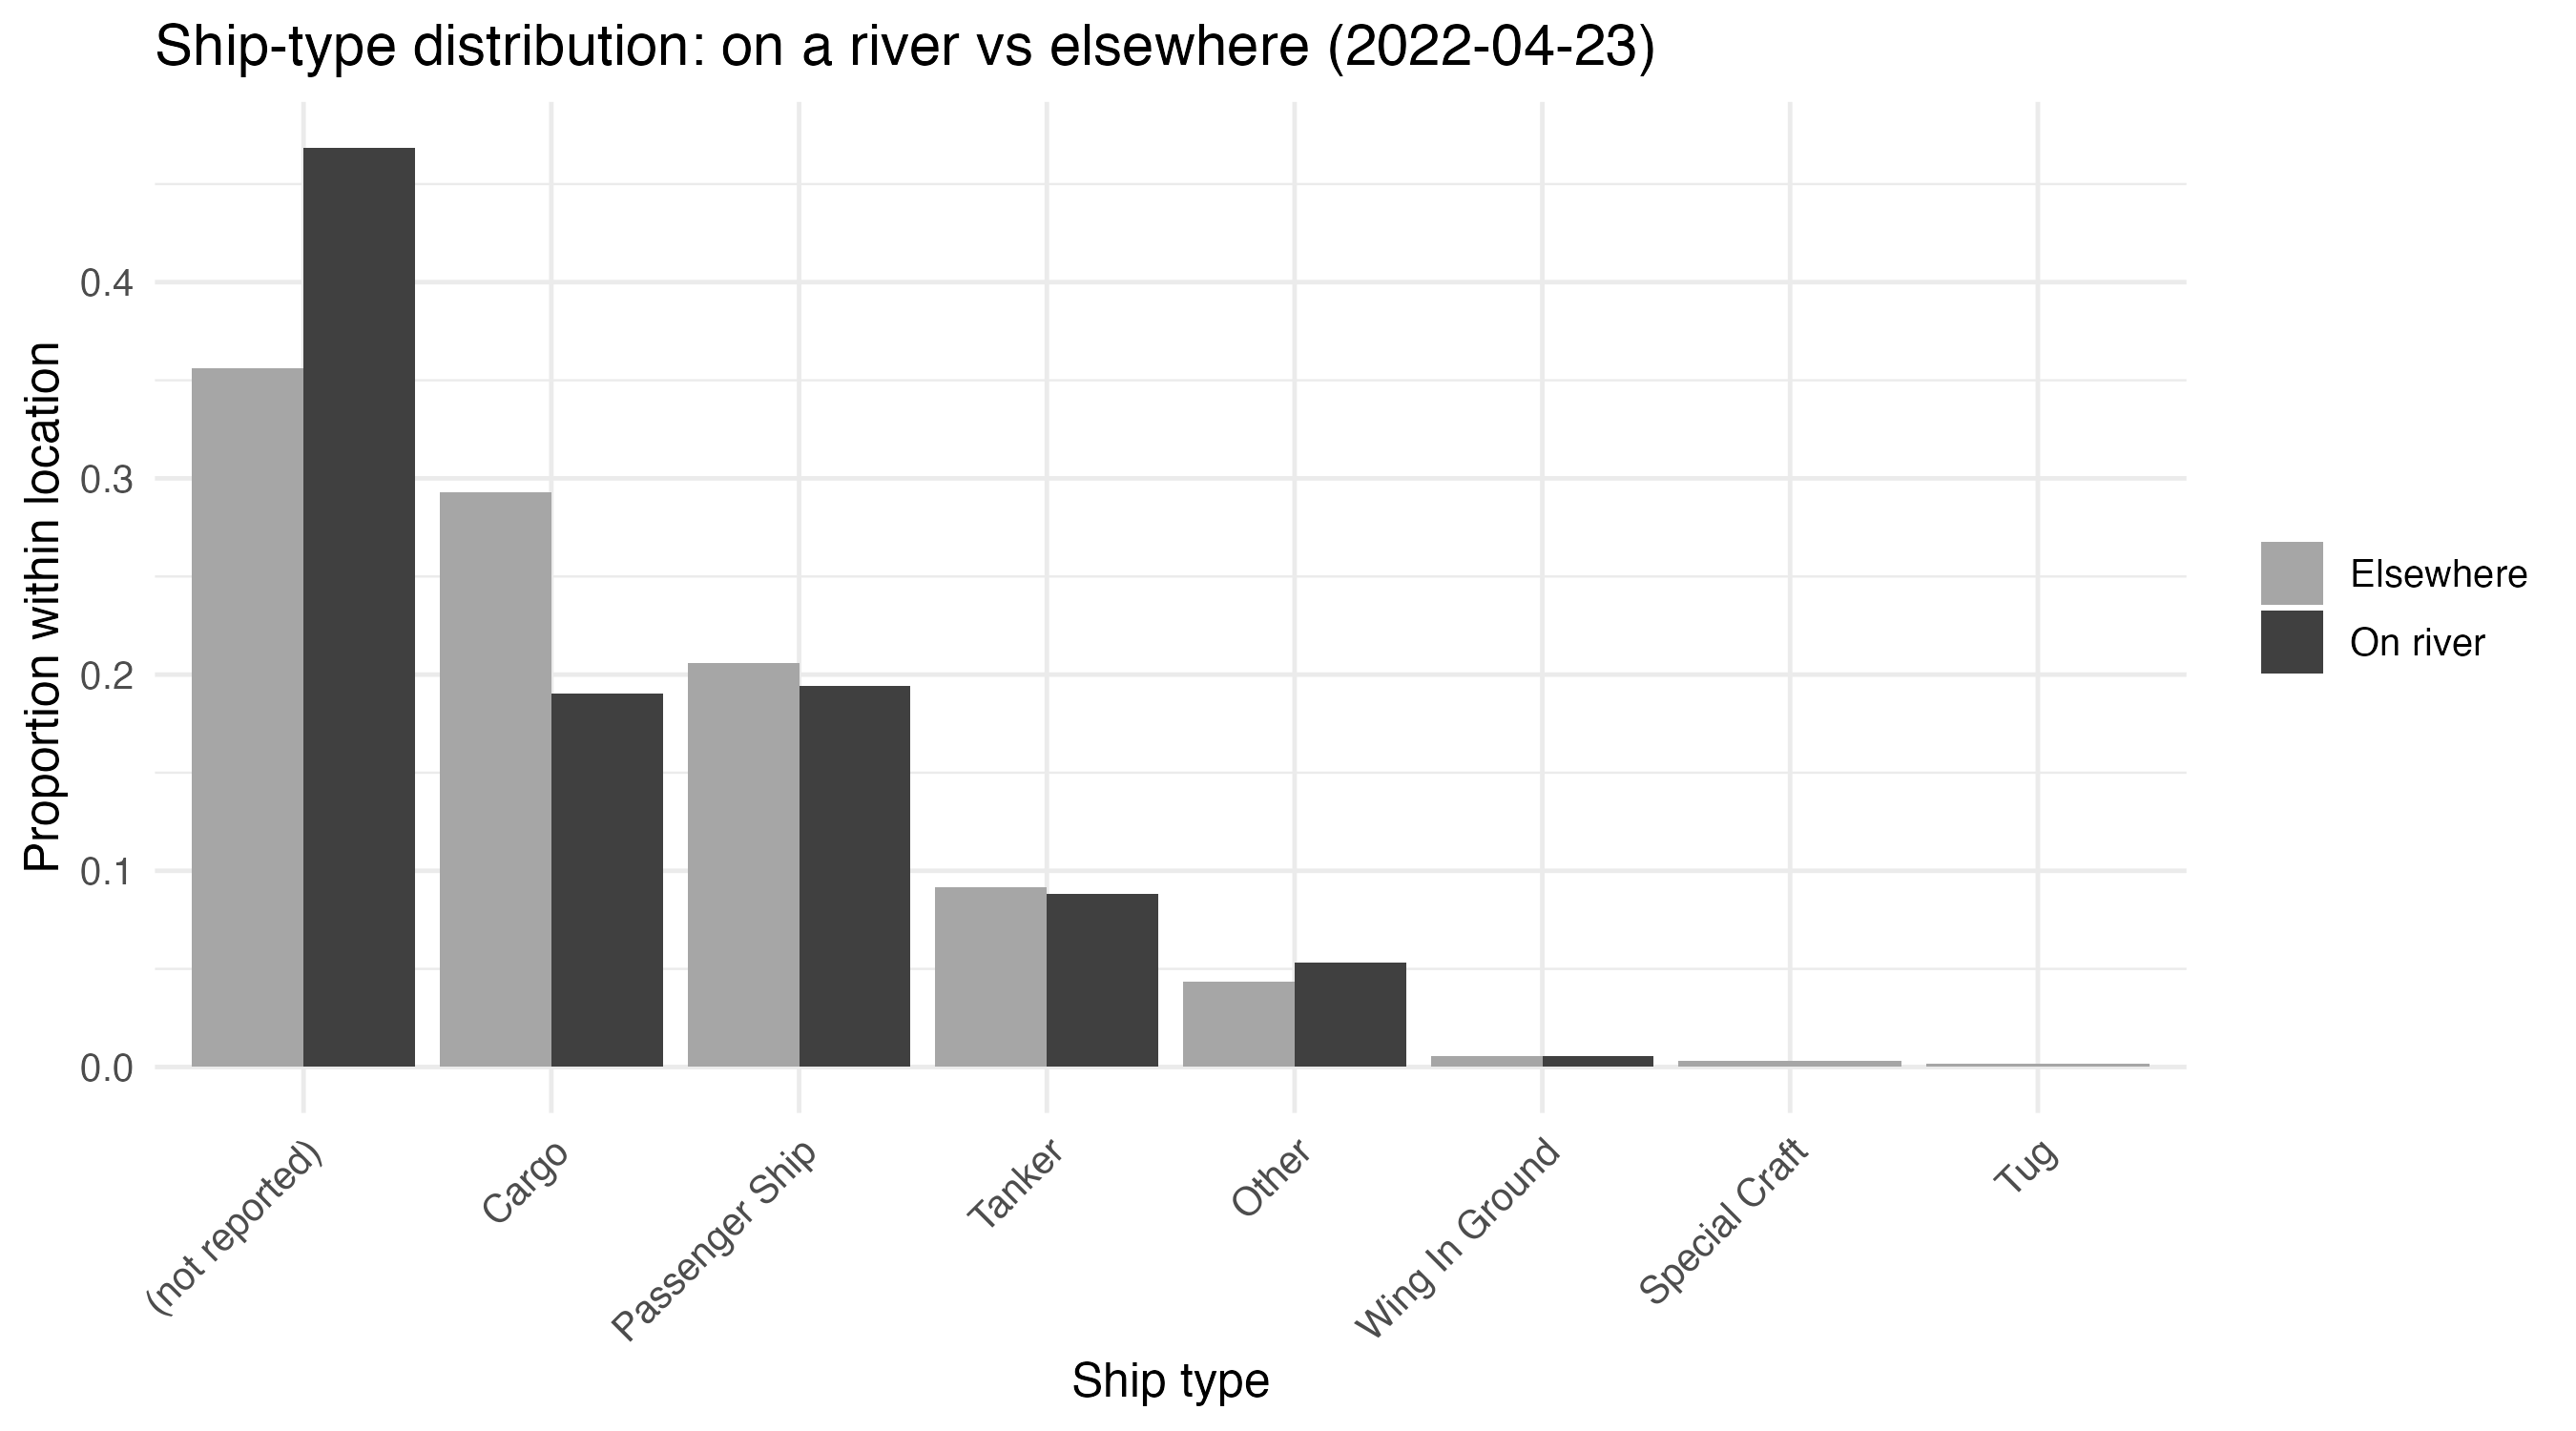
\includegraphics[width=0.85\textwidth]{rivertype_vs_elsewhere.png}
    \caption{\textbf{Ship types on rivers vs.\ elsewhere.} Share of each ship type among records matched to a German river compared with those tracked elsewhere (2022-04-23).}
    \label{fig:rivertype}
\end{figure}

Aggregating the on-river records by river gives the ranking in
Table~\ref{tab:river-records}. The Rhine carries by far the most traffic with 89,033
records, followed by the Elbe (62,680) and the Weser (20,362); the remaining rivers
each account for a few thousand records or fewer. The Inn and Oder, although they
contribute H3 cells, returned no matched records on this date and are therefore not
listed, which is plausible given their limited and largely border-bound inland AIS
coverage.

\begin{table}[ht]
\caption{\textbf{AIS records per German river (2022-04-23).} Matched record count per river, in descending order.}
\label{tab:river-records}
\vspace{0.2cm}
\centering
\small
\begin{tabular}{@{}lr@{}}
\toprule
{\bfseries River} & {\bfseries AIS records} \\
\midrule
Rhine & 89,033 \\
Elbe  & 62,680 \\
Weser & 20,362 \\
Donau &  3,895 \\
Main  &  3,768 \\
Mosel &  2,510 \\
Ems   &  1,160 \\
\bottomrule
\end{tabular}
\end{table}

Finally, the distribution of traffic \emph{along} the Rhine was examined in more
detail. The 89,033 Rhine records were projected onto the Rhine geometry to obtain each
point's distance along the river, which was then binned into 10~km intervals;
Figure~\ref{fig:rhine} shows the resulting density. This step requires two assumptions
about the reference geometry. First, the clipped German Rhine consists of several
disconnected pieces, so a single continuous reference line was constructed by orienting
each piece from north to south and joining the pieces in order of latitude; because the
joined line bridges the gaps between pieces, the resulting distance scale (about
1,078~km) somewhat overstates the true navigable channel and should be read as a
relative position along the river rather than exact kilometrage. Second, distance is
measured from the northernmost point southward, so 0~km corresponds to the lower Rhine
near the Dutch border and increasing values move upstream. With these assumptions, the
plot shows traffic concentrated in distinct stretches rather than spread evenly, with
pronounced peaks that correspond to the busier lower- and middle-Rhine reaches.

\begin{figure}[H]
    \centering
    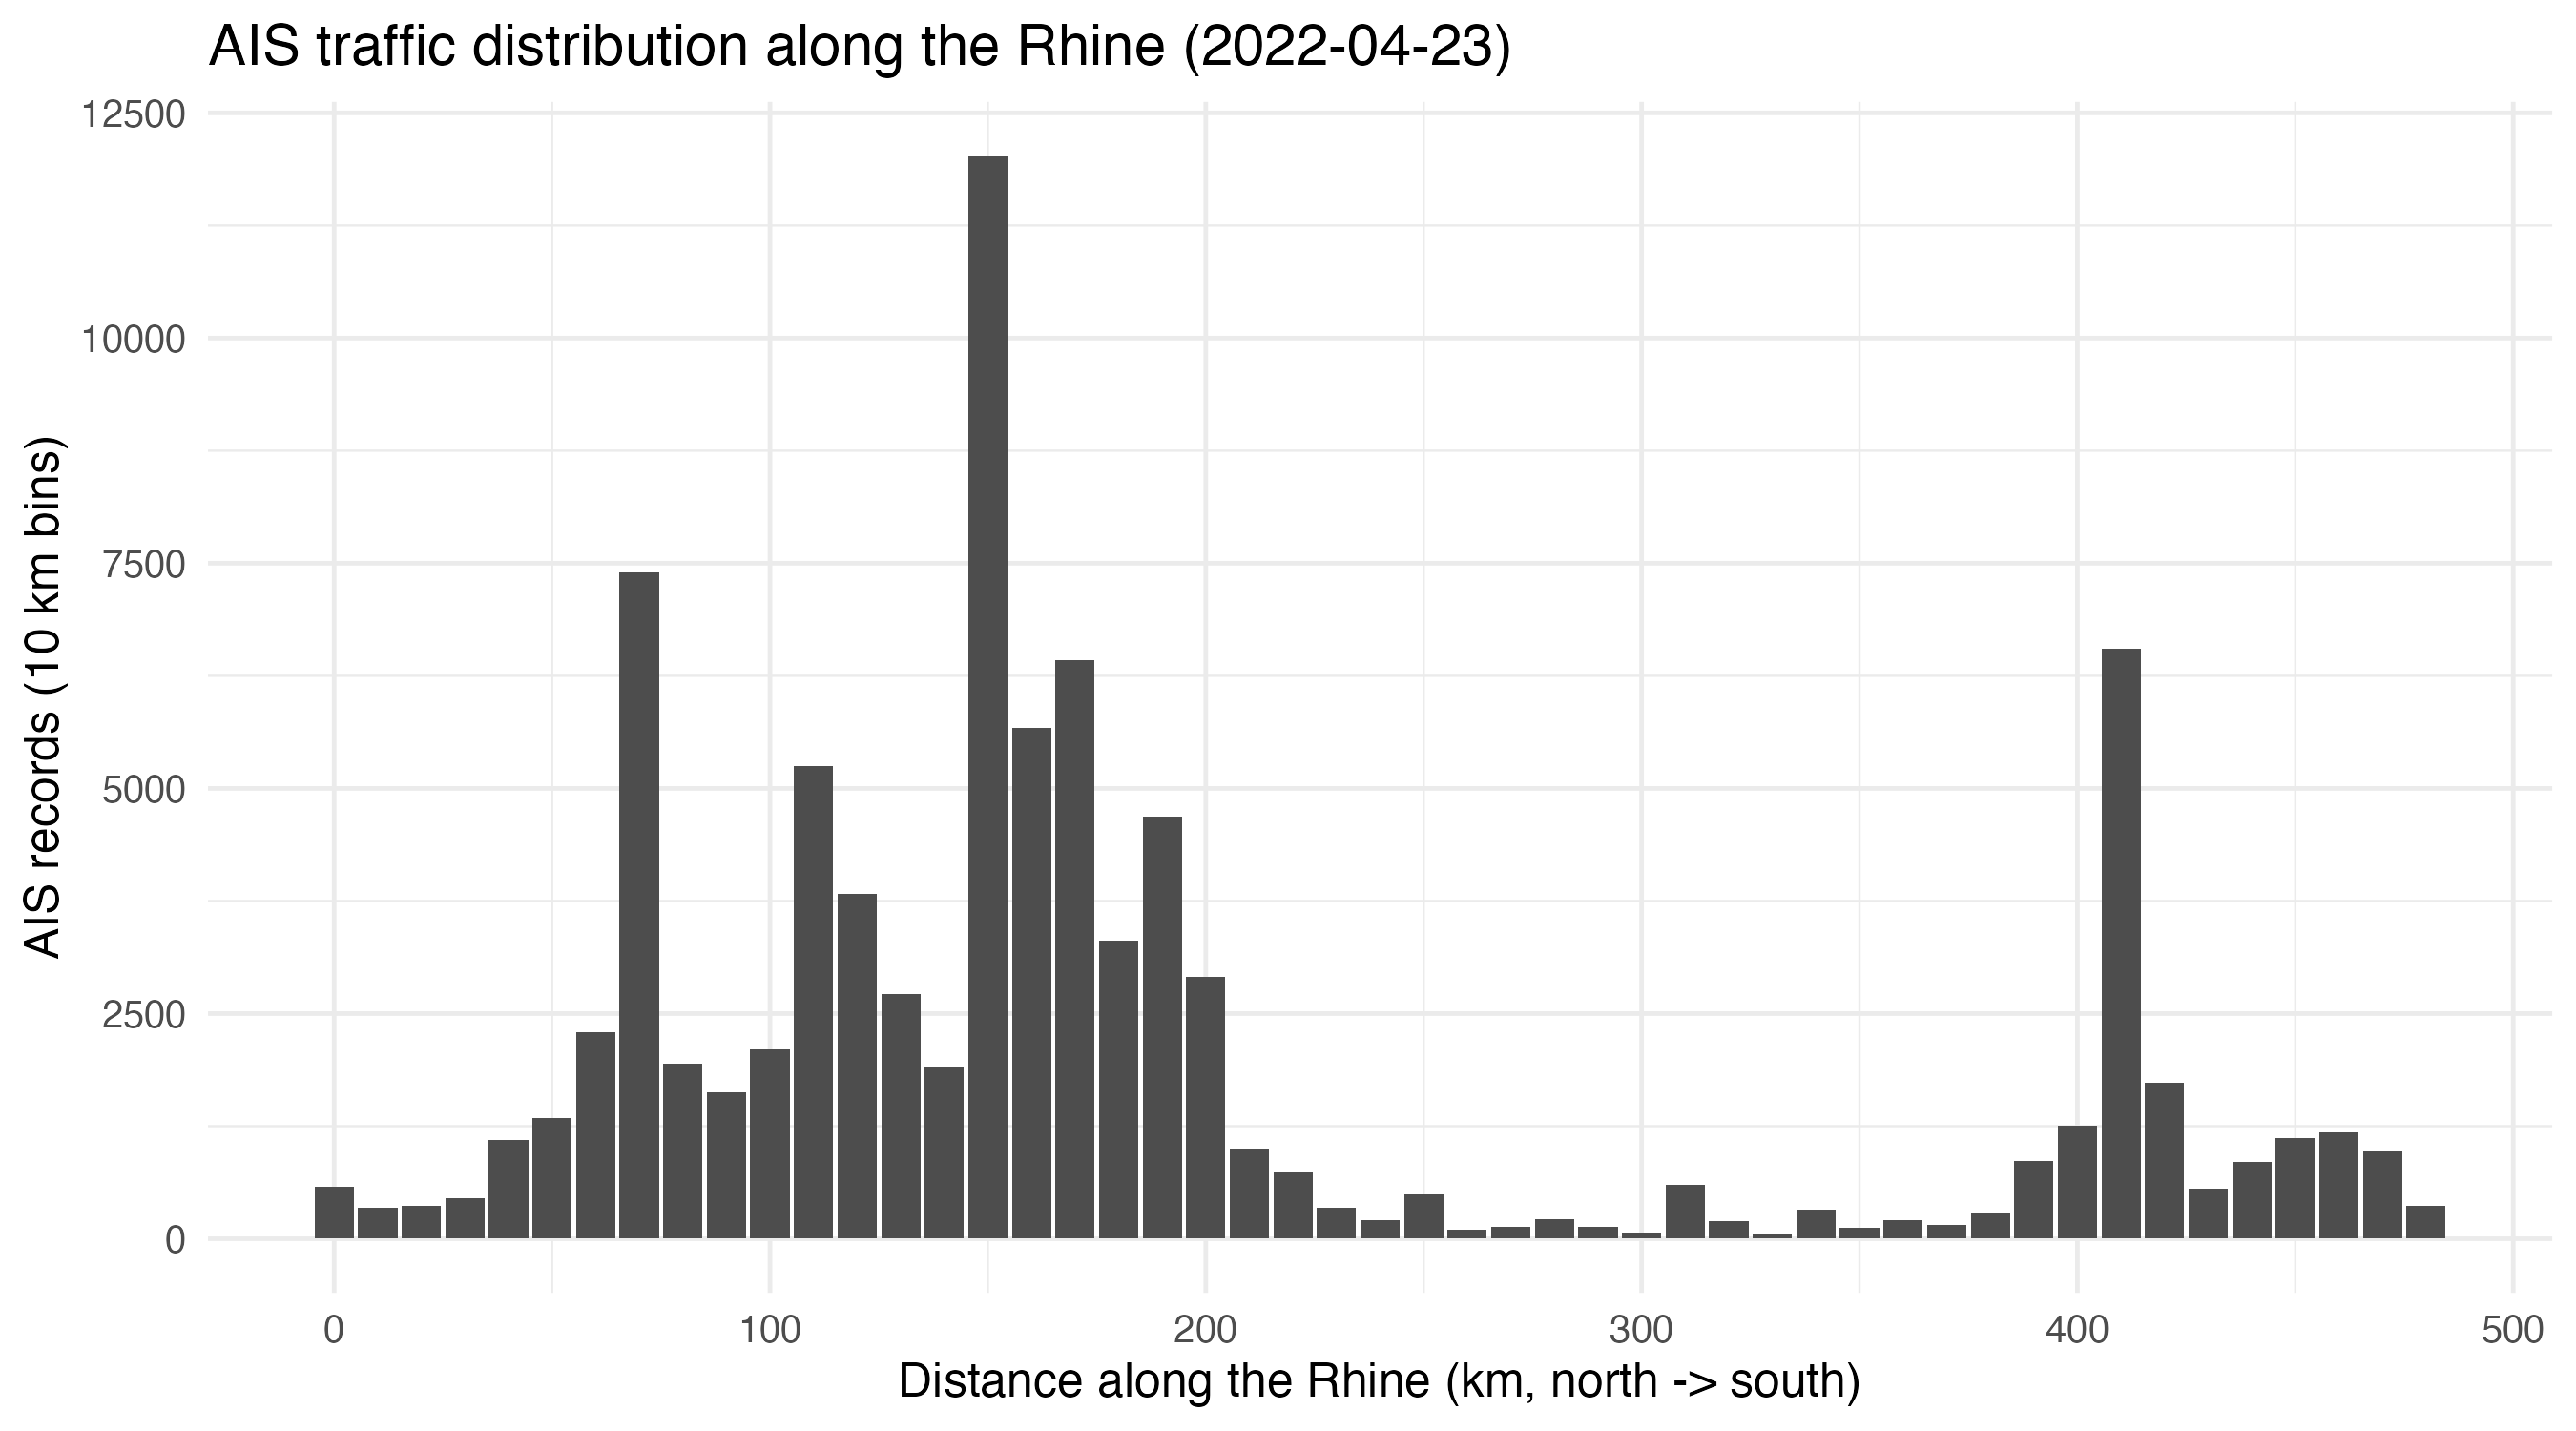
\includegraphics[width=0.85\textwidth]{rhine_distribution.png}
    \caption{\textbf{Traffic distribution along the Rhine.} AIS records in 10~km bins (2022-04-23), measured north to south.}
    \label{fig:rhine}
\end{figure}

% ======================================================================================
% 7. Dashboard and Deployment Evidence
% ======================================================================================

\section {Dashboard and Deployment Evidence}

Both web components are deployed on the assigned server through a single Docker
Compose stack (an NGINX container and a Shiny container on a shared network) and
are reachable behind the NGINX reverse proxy.

The \textbf{static dashboard} is the speed-coloured interval-sample map from
Section~5, exported as a self-contained HTML page
(\texttt{02\_code/R/sample\_html\_dashboard.R} via
\texttt{htmlwidgets::saveWidget()}) and served from the NGINX document root. A
reader sees the 10{,}000 sampled AIS positions as circle markers coloured by
speed over ground (capped at 25 knots; pale yellow $=$ slow, dark red $=$ fast),
clustered at low zoom for legibility, with a speed legend.

The \textbf{interactive Shiny application} reuses the river traffic-density logic
from Section~6. The user selects a river and one or more ship types and clicks
\texttt{refresh} to update the traffic-density plot for 2022-04-23. To avoid
repeated expensive API calls from the deployed app, the required data are
pre-computed once \texttt{02\_code/R/prepare\_shiny\_data.R} and written to a
CSV that the app reads at start-up. NGINX exposes the app under the
\texttt{/ais\_app} endpoint.

\begin{table}[h]
    \centering
    \caption{\textbf{Dashboard and deployment evidence.} The two deployed web components and where each can be verified.}
    \label{tab:deploy}
    \begin{tabular}{l p{9.5cm}}
        \toprule
        \textbf{Component} & \textbf{Evidence} \\
        \midrule
        Static map dashboard &
        Live at \url{http://193.197.231.174:7080/sample_points.html};
        see Figure~\ref{fig:dash}. \\
        Interactive Shiny application &
        Live at \url{http://193.197.231.174:7080/ais_app/};
        see Figure~\ref{fig:shiny}. \\
        \bottomrule
    \end{tabular}
\end{table}

\begin{figure}[H]
    \centering
    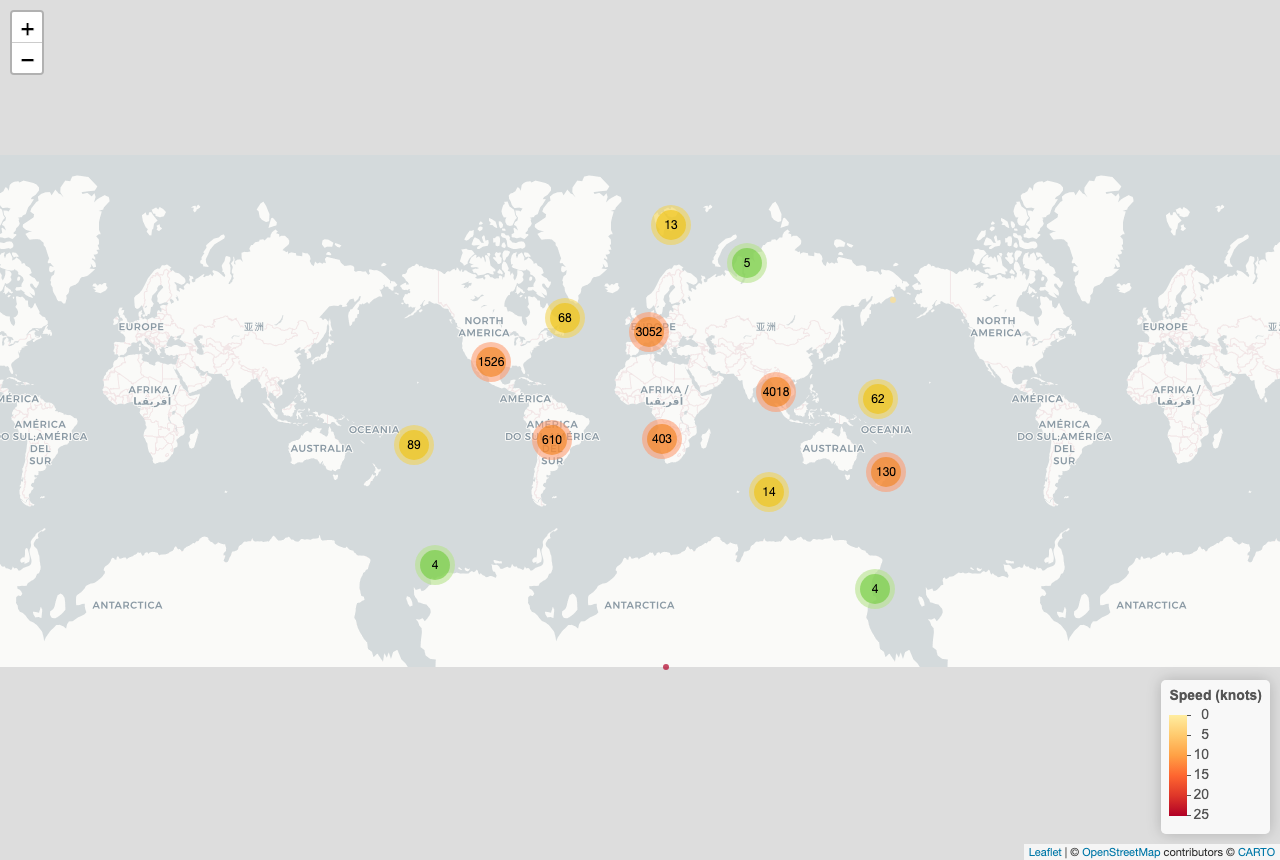
\includegraphics[width=0.85\textwidth]{dashboard_deployed.png}
    \caption{\textbf{Deployed static dashboard.} The speed-coloured sample map served by NGINX under \texttt{/sample\_points.html}.}
    \label{fig:dash}
\end{figure}

\begin{figure}[H]
    \centering
    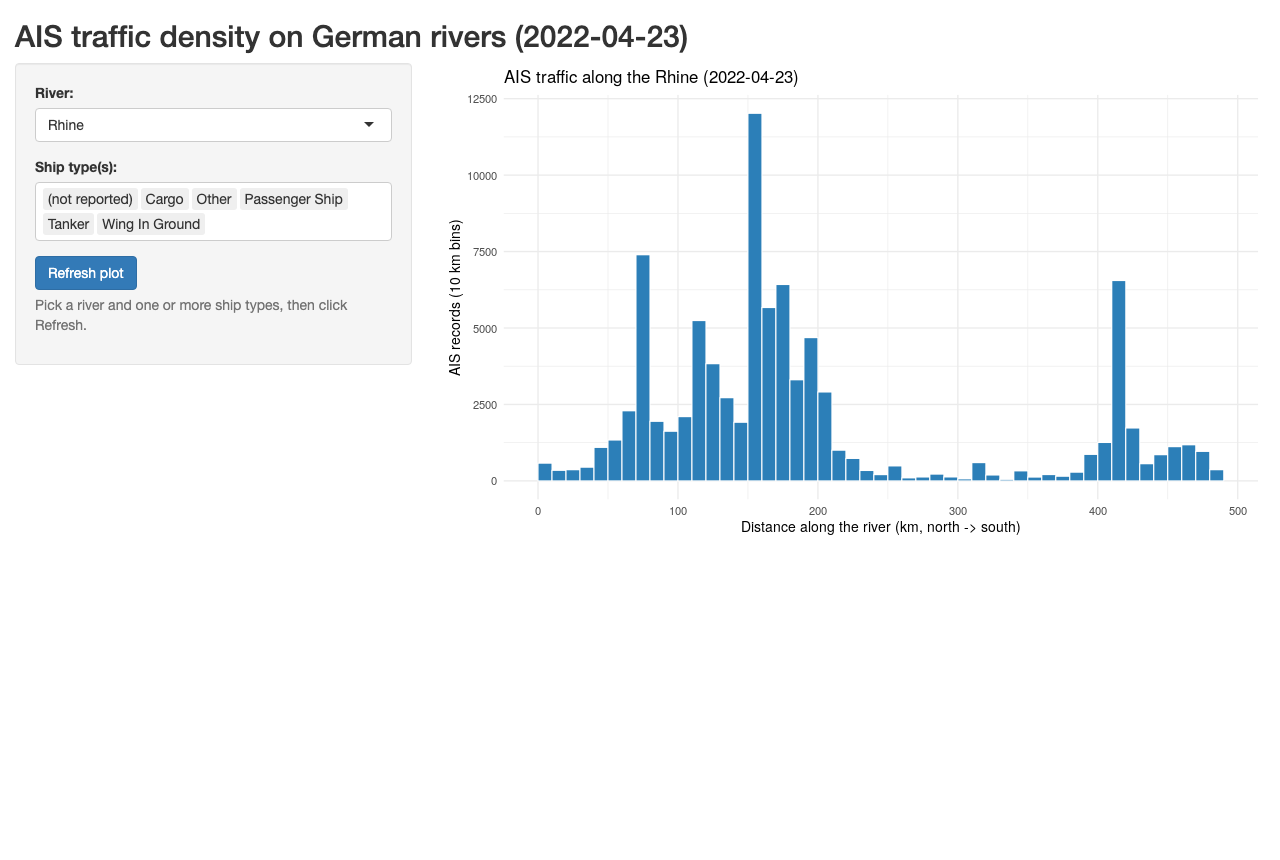
\includegraphics[width=0.85\textwidth]{shiny_deployed.png}
    \caption{\textbf{Deployed Shiny application.} The interactive river traffic-density app served under \texttt{/ais\_app}.}
    \label{fig:shiny}
\end{figure}

Both endpoints were confirmed to load and respond in a browser; the Shiny inputs
update the plot when the \texttt{refresh} button is clicked.


% ======================================================================================
% 8. Conclusion
% ======================================================================================

\section {Conclusion}

This report examined the analytical potential and the limitations of AIS data for the
study of vessel movement. After introducing how AIS data are generated, transmitted,
and collected, the descriptive overview showed that the database is large but uneven:
key fields such as draught or destination are frequently missing or contain
placeholder values, and the data are concentrated on a few ship types, flags, and
regions, reflecting both SOLAS carriage rules and coverage-dependent reception.

Because the full dynamic table is far too large to analyse directly, two sampling
strategies were compared. The interval (cluster) sample proved easy to construct but
sensitive to the randomly chosen time windows, over-representing slow and stationary
vessels, whereas the stratified sample preserved the structure of ship types and hours
more faithfully and was therefore the more representative basis for analysis. The
vessel-behaviour analysis then illustrated, on individual tracks, both a clear
data-quality failure (a shared or default MMSI producing a physically impossible
worldwide track) and characteristic real patterns (a vessel idle at berth in
Constan\c{t}a, and a Danube voyage whose ship-lock passages were recovered by a simple,
transparent low-speed clustering heuristic). Combining the AIS records with river
geometries through H3 spatial indexing showed that about 37\% of German traffic on the
study date ran on the inland river network, dominated by the Rhine and the Elbe.
Finally, the results were made accessible through a deployed static dashboard and an
interactive Shiny application.

Overall, the project demonstrates that AIS data support rich analyses of maritime and
inland traffic, but only when their gaps, biases, and errors are handled explicitly:
through deliberate sampling, plausibility-aware interpretation, and transparent,
reproducible processing. The same coverage and quality limitations that shape the
results also mark the natural directions for future work, such as multi-day analyses,
more sophisticated (for example unsupervised) event detection, and systematic data
cleaning before interpretation.

% ======================================================================================
% 9. Declaration on the Use of AI Tools
% ======================================================================================

\section {Declaration on the Use of AI Tools}

Claude (Anthropic), via the Claude Code CLI, was used as a coding and writing
assistant: drafting and editing report sections, constructing and debugging the
PostgREST queries and R scripts, and configuring the Docker/NGINX deployment.
All code and text were reviewed, tested, and validated by us, and the analytical
decisions and the interpretation of results remain our own. No AI-generated
citations were used without checking the original sources.

% ======================================================================================
% References
% ======================================================================================

\begin{thebibliography}{13}

\bibitem{1}
NATO Shipping Centre, 2021,
``AIS (Automatic Identification System) Overview'',
\url{https://shipping.nato.int/nsc/media-centre/news-archive/2021/ais-automatic-identification-system-overview}
(Accessed: 2026-06-16).

\bibitem{2}
S. Kos, L. Vojkovi{\'c}, and D. Br{\v{c}}i{\'c}, 2014,
``Development of AIS and its Influence on Marine Traffic Control'',
\url{https://www.researchgate.net/publication/333802094_Development_of_AIS_and_its_influence_on_marine_traffic_control}

\bibitem{3}
International Maritime Organization,
``AIS transponders'',
\url{https://www.imo.org/en/OurWork/Safety/Pages/AIS.aspx}
(Accessed: 2026-06-16)

\bibitem{4}
T. Eriksen, G. H{\o}ye, B. Narheim, and B. J. Meland, 2006,
``Maritime traffic monitoring using a space-based AIS receiver'',
\url{https://www.sciencedirect.com/science/article/pii/S0094576506000233}

\bibitem{5}
G. Wang, L. Li, X. Chen, Z. Zhang, 2026,
``Deep Learning-Based AIS Signal Collision Detection in Satellite Reception Environment '',
\url{https://www.mdpi.com/2076-3417/16/2/643}

\bibitem{6}
Y. Yang, Y. Liu, G. Li, Z. Zhang, Y. Liu, 2024,
``Harnessing the power of Machine learning for AIS Data-Driven maritime Research: A comprehensive review'',
\url{https://www.sciencedirect.com/science/article/pii/S1366554524000164\#b0175}

\bibitem{7}
T. Emmens, C. Amrit, A. Abdi, M. Ghosh, 2021,
``The promises and perils of Automatic Identification System data'',
\url{https://www.sciencedirect.com/science/article/pii/S0957417421004164}

\bibitem{8}
Catalogue of Bias, 2019,
``Availability bias'',
\url{https://catalogofbias.org/biases/availability-bias/}
(Accessed: 2026-06-17)

\bibitem{9}
W. He, J. Lei, X. Chu, S. Xie, C. Zhong, Z. Li, 2021,
``A Visual Analysis Approach to Understand and Explore Quality Problems of AIS Data'',
\url{https://www.mdpi.com/2077-1312/9/2/198}

\bibitem{10}
L. Zhao, G. Shi, J. Yang, 2018,
``Ship Trajectories Pre-processing Based on AIS Data'',
\url{https://www.cambridge.org/core/journals/journal-of-navigation/article/ship-trajectories-preprocessing-based-on-ais-data/4F5B73157D600B2821CB698FDE3C24A7}

\bibitem{11}
J. Fan, F. Han, H. Liu, 2014,
``Challenges of Big Data Analysis'',
\url{https://pmc.ncbi.nlm.nih.gov/articles/PMC4236847}

\bibitem{12}
GeeksforGeeks,
``Introduction to Data Sampling'',
\url{https://www.geeksforgeeks.org/data-analysis/what-is-data-sampling/}
(Accessed: 2026-06-18)

\bibitem{13}
Uber Technologies, 2025,
``H3: Hexagonal Hierarchical Geospatial Indexing System -- Documentation'',
\url{https://h3geo.org/docs/}
(Accessed: 2026-06-19)

\end{thebibliography}

% =============================================================================
%  APPENDIX
% =============================================================================

\section*{A Appendix: Reproducibility and Repository Information}

\label{app:repro}

This appendix collects the technical information needed to reproduce the results,
kept here rather than in the main narrative. A full, file-by-file description of
the repository and the run instructions is given in the \texttt{README.md} at the
repository root.

\subsection*{A.1 Repository Structure}

The submission follows the folder structure required in Task~1:
\begin{itemize}
    \item \texttt{00\_docs} --- assignment sheet and supporting documents.
    \item \texttt{01\_data} --- generated samples and cached intermediate data
          products.
    \item \texttt{02\_code/R} --- analysis scripts, with reusable helpers in
          \texttt{functions/}.
    \item \texttt{03\_report} --- this report and, in \texttt{graphs/}, every
          figure it uses.
\end{itemize}
The deployment files (\texttt{docker-compose.yaml}, \texttt{nginx/},
\texttt{shiny/}, \texttt{www/}) live at the repository root and are described in
the \texttt{README.md}.

\subsection*{A.2 Execution Order and Reproduction Notes}

All scripts use paths relative to the repository root; opening
\texttt{aidaho\_ids\_thas\_2026.Rproj} in RStudio sets the working directory
accordingly. Random samples use a fixed seed (\texttt{set.seed(2026)}), and large
API results are cached as \texttt{.rds} files in \texttt{01\_data/}, so a re-run
uses the cache instead of re-querying the shared database. The per-script task
mapping, and the three scripts that require live API access, are listed in the
\texttt{README.md}.

\begin{table}[h]
    \centering
    \caption{\textbf{Technical reproduction overview.} Main input and output of each analysis step.}
    \label{tab:repro}
    \begin{tabular}{p{3cm} p{4.3cm} p{6.2cm}}
        \toprule
        \textbf{Analysis step} & \textbf{Main input} & \textbf{Main output} \\
        \midrule
        Data overview       & AIS database (PostgREST)                & overview tables \\
        Sample construction & \texttt{ais\_dynamic} messages          & \texttt{sample\_intervals.csv}, \texttt{sample\_stratified.csv} \\
        Vessel behaviour    & selected AIS tracks                     & vessel maps, lock-event table \\
        River traffic       & \texttt{ais\_germany}, river geometries & river-traffic figures \\
        Deployment          & prepared CSV                            & static dashboard, Shiny app \\
        \bottomrule
    \end{tabular}
\end{table}

\subsection*{A.3 Software Environment}

\begin{table}[h]
    \centering
    \caption{\textbf{Software environment.} Versions and tools used to produce the submitted results.}
    \label{tab:software}
    \begin{tabular}{l p{10.5cm}}
        \toprule
        \textbf{Component} & \textbf{Version or description} \\
        \midrule
        R version          & 4.6.0 (2026-04-24) \\
        Operating system   & macOS 26.5 (Apple silicon, \texttt{aarch64}) \\
        Package management & \texttt{install.packages()}; no \texttt{renv} lockfile. The required packages and the install command are listed in the \texttt{README.md}. \\
        Deployment         & Docker Compose (NGINX + Shiny) \\
        \bottomrule
    \end{tabular}
\end{table}

\subsection*{A.4 Important Submitted Files}

\begin{itemize}
    \item \texttt{README.md} --- repository overview and run instructions.
    \item \texttt{01\_data/sample\_intervals.csv} --- interval (cluster) sample (Task~3.2).
    \item \texttt{01\_data/sample\_stratified.csv} --- stratified sample (Task~3.3).
    \item \texttt{03\_report/graphs/} --- all figures used in this report.
    \item \texttt{docker-compose.yaml}, \texttt{shiny/}, \texttt{nginx/},
          \texttt{www/} --- WebApp deployment (Tasks~6--7).
\end{itemize}

\end{document}